\documentclass[aspectratio=169,10pt]{beamer}

% Modern professional theme for computer vision presentation
\usetheme{metropolis}
\usecolortheme{default}

% Custom color scheme optimized for computer vision presentation
\definecolor{primaryblue}{RGB}{20,75,140}
\definecolor{secondaryblue}{RGB}{70,130,180}
\definecolor{accentorange}{RGB}{230,95,45}
\definecolor{lightgray}{RGB}{245,245,245}
\definecolor{darkgray}{RGB}{45,45,45}

% Metropolis color customization
\setbeamercolor{progress bar}{fg=primaryblue,bg=lightgray}
\setbeamercolor{title separator}{fg=primaryblue}
\setbeamercolor{progress bar in head/foot}{fg=primaryblue}
\setbeamercolor{progress bar in section page}{fg=primaryblue}
\setbeamercolor{frametitle}{bg=primaryblue,fg=white}
\setbeamercolor{title}{fg=primaryblue}
\setbeamercolor{subtitle}{fg=secondaryblue}
\setbeamercolor{structure}{fg=primaryblue}
\setbeamercolor{alerted text}{fg=accentorange}
\setbeamercolor{block title}{bg=primaryblue,fg=white}
\setbeamercolor{block body}{bg=lightgray,fg=darkgray}
\setbeamercolor{block title alerted}{bg=accentorange,fg=white}
\setbeamercolor{block body alerted}{bg=lightgray,fg=darkgray}

% Enhanced packages for mathematical rigor
\usepackage{amsmath,amssymb,amsfonts}
\usepackage{graphicx}
\usepackage{booktabs}
\usepackage{xcolor}
\usepackage{tikz}
\usepackage{algorithm2e}

% Professional formatting
\setbeamertemplate{navigation symbols}{}
\setbeamertemplate{footline}[frame number]

% Title information
\title{Computer Vision \& Deep Learning I}
\subtitle{CMSC 178IP - Digital Image Processing}
\author{Noel Jeffrey Pinton}
\institute{University of the Philippines - Cebu\\Department of Computer Science}
\date{}

% Adjust title page spacing
\setbeamertemplate{title page}[default][colsep=-4bp,rounded=true]

\begin{document}

% Title slide
\begin{frame}
\titlepage
\end{frame}

% Table of contents
\begin{frame}[shrink=10]{Course Outline}
\tableofcontents
\end{frame}

\section{Introduction to Neural Networks}

\begin{frame}{What is Deep Learning?}
\begin{alertblock}{Definition}
Deep Learning is a subset of machine learning based on artificial neural networks with multiple layers that progressively extract higher-level features from raw input.
\end{alertblock}

\textbf{Key Characteristics:}
\begin{itemize}
\item Hierarchical feature learning
\item End-to-end learning from data
\item Automatic feature extraction
\item Scalability with data and compute
\end{itemize}

\textbf{Applications in Computer Vision:}
\begin{itemize}
\item Image classification
\item Object detection and localization
\item Semantic segmentation
\item Image generation and enhancement
\end{itemize}
\end{frame}

\begin{frame}{Evolution of Computer Vision}
\begin{columns}
\column{0.5\textwidth}
\textbf{Traditional Approach:}
\begin{itemize}
\item Hand-crafted features (SIFT, HOG)
\item Classical ML classifiers (SVM, RF)
\item Limited representation capacity
\item Manual feature engineering
\end{itemize}

\textbf{Deep Learning Approach:}
\begin{itemize}
\item Learned hierarchical features
\item End-to-end optimization
\item Superior performance
\item Data-driven representations
\end{itemize}

\column{0.45\textwidth}
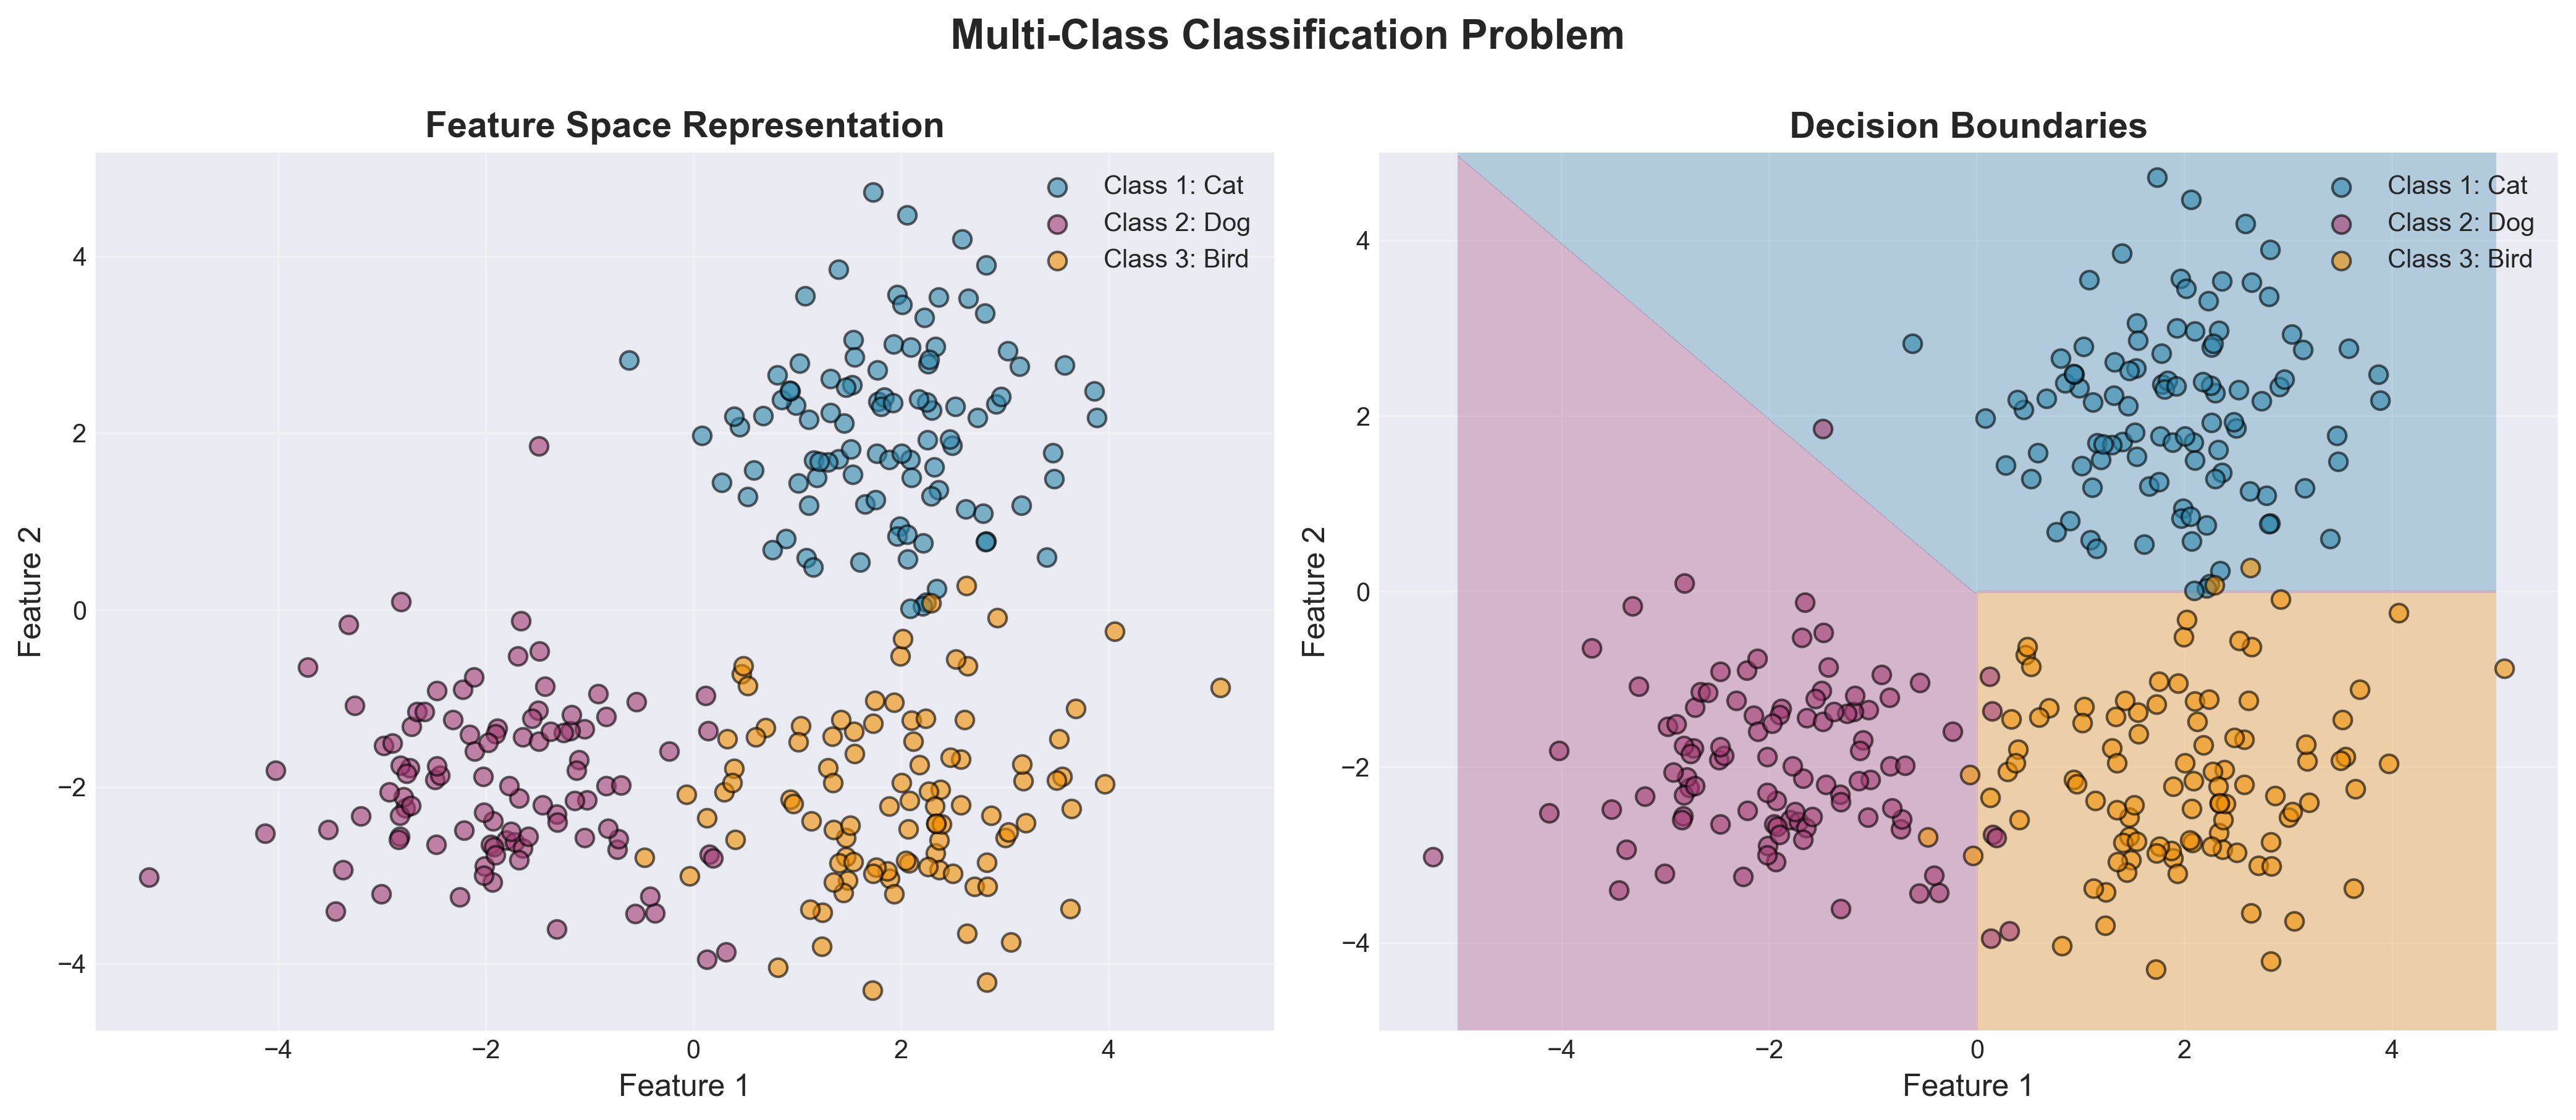
\includegraphics[width=\textwidth]{../figures/13_classification_example.png}\\
\centering{\small Modern deep learning classification pipeline}
\end{columns}
\end{frame}

\section{Perceptrons and Neural Networks}

\begin{frame}{The Perceptron}
\begin{columns}
\column{0.5\textwidth}
\begin{alertblock}{Perceptron Model}
The perceptron is the fundamental building block of neural networks.
\end{alertblock}

\textbf{Mathematical Formulation:}
$$y = f\left(\sum_{i=1}^{n} w_i x_i + b\right) = f(\mathbf{w}^T\mathbf{x} + b)$$

Where:
\begin{itemize}
\item $\mathbf{x} = [x_1, x_2, \ldots, x_n]^T$ = input features
\item $\mathbf{w} = [w_1, w_2, \ldots, w_n]^T$ = weights
\item $b$ = bias term
\item $f(\cdot)$ = activation function
\end{itemize}

\column{0.45\textwidth}
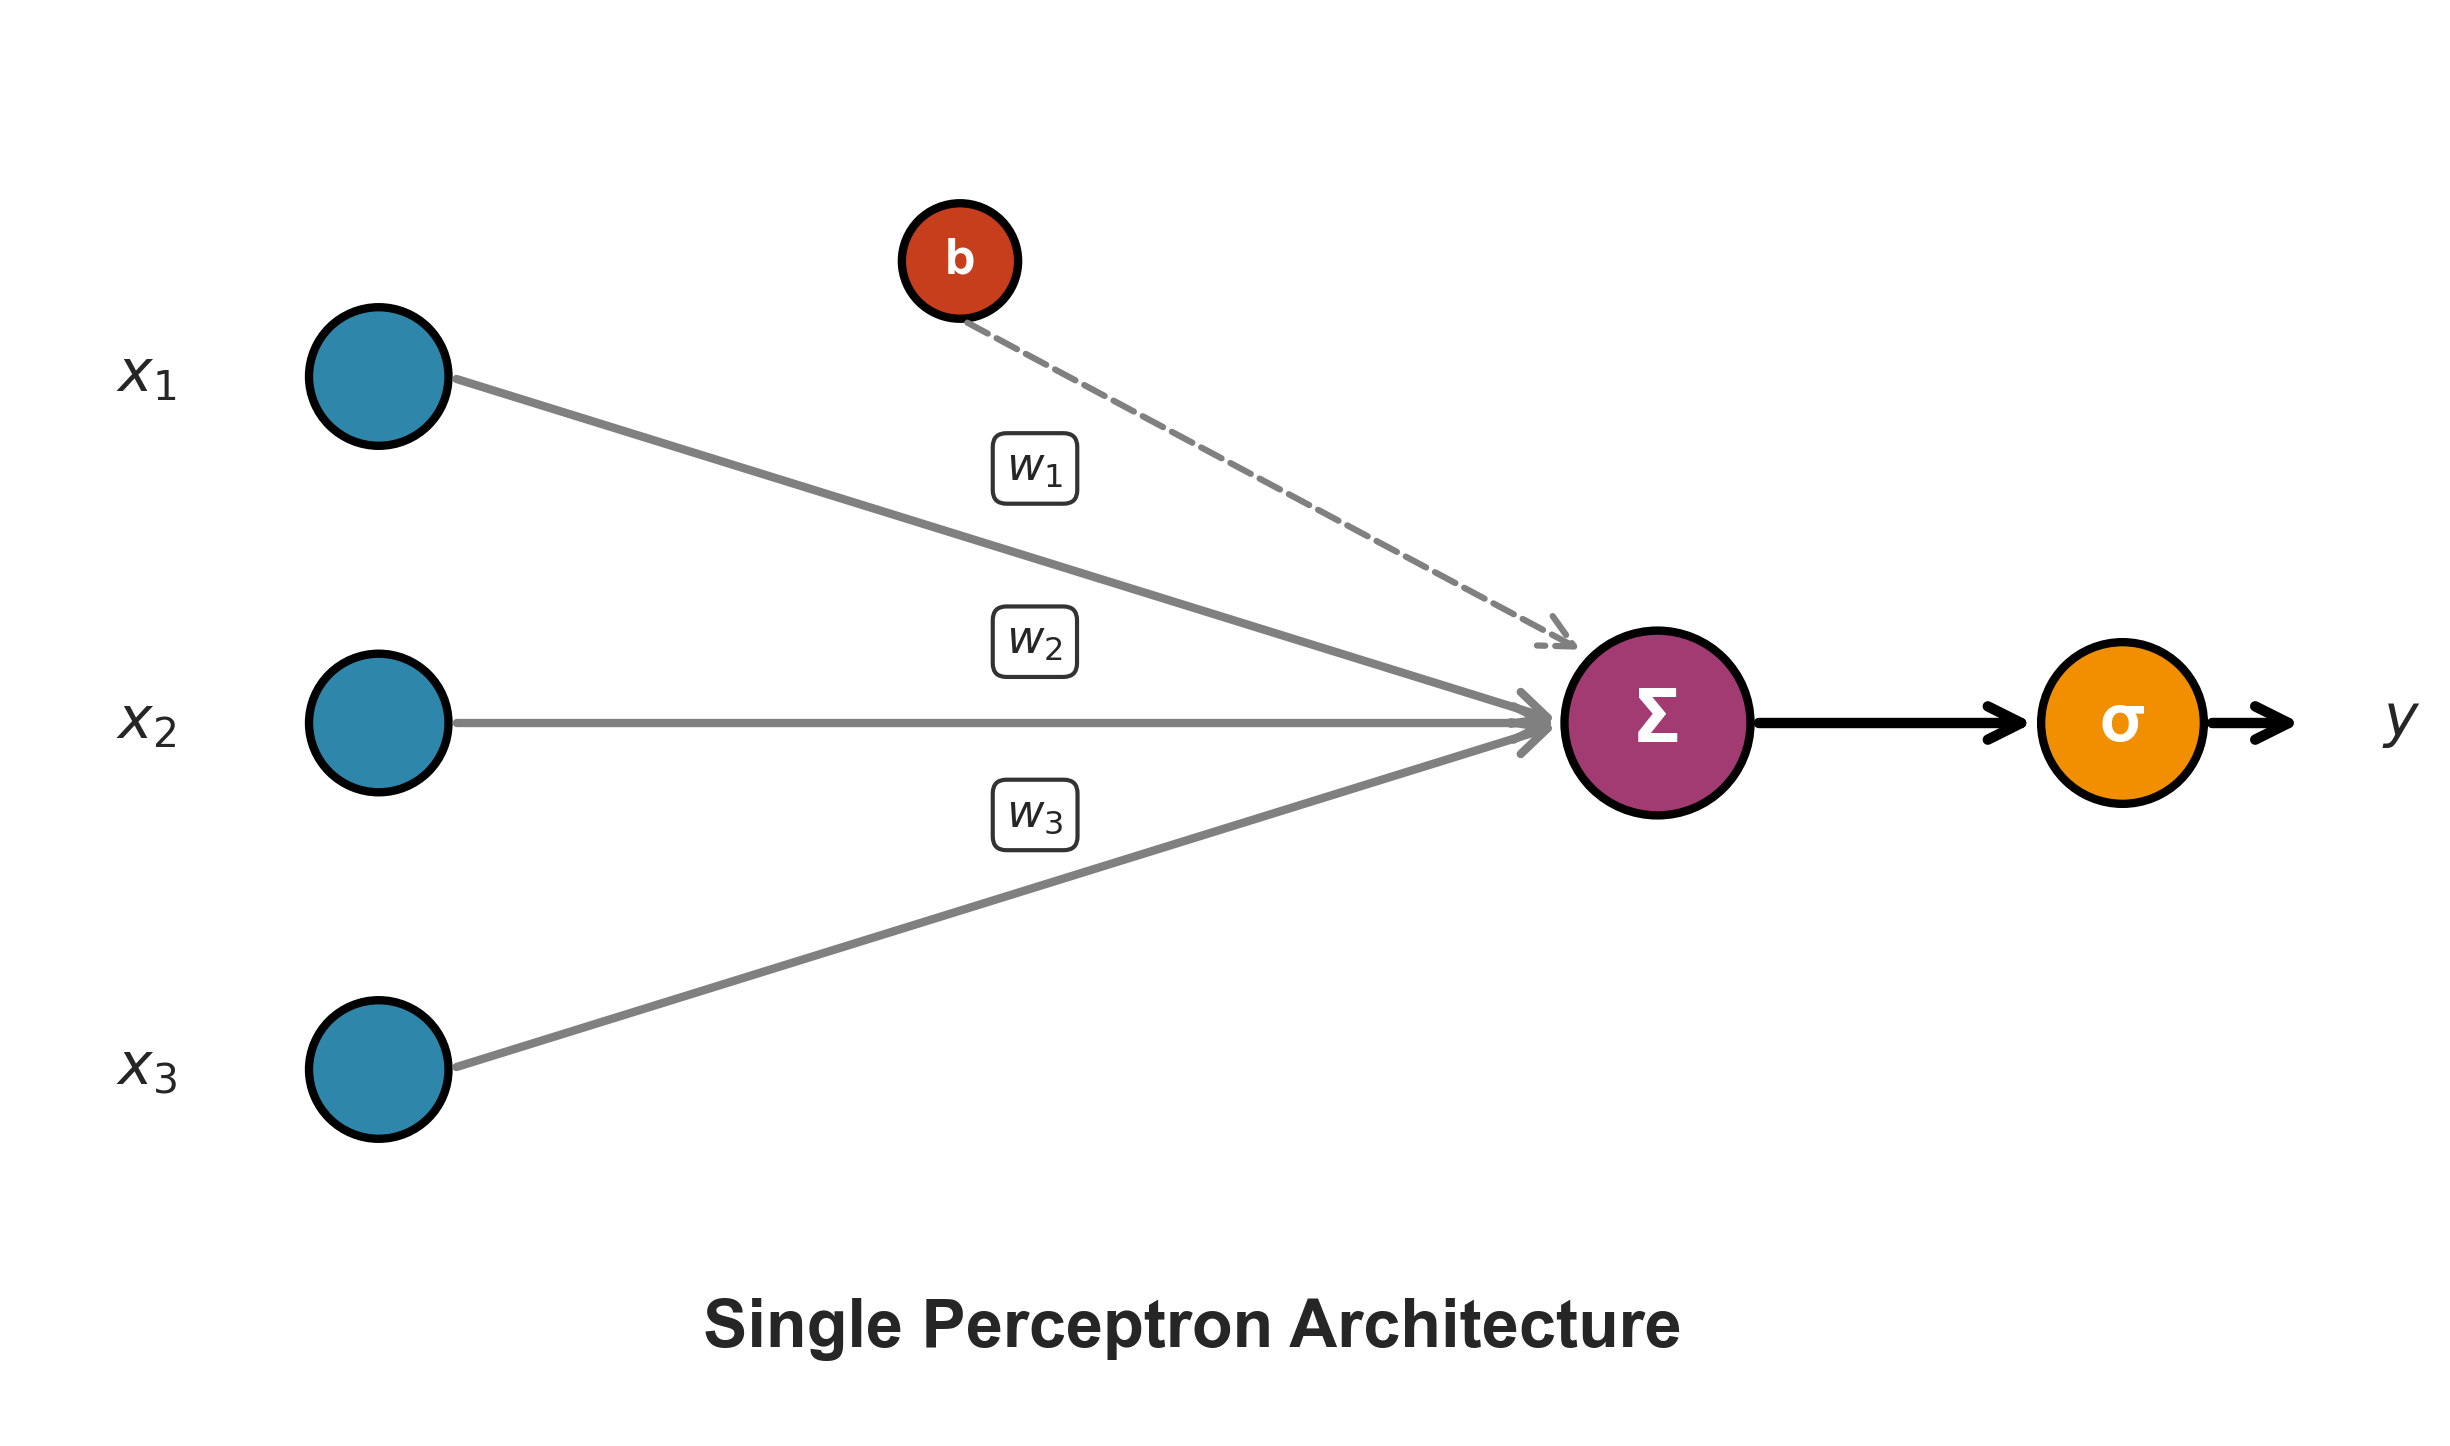
\includegraphics[width=\textwidth]{../figures/02_perceptron_diagram.png}\\
\centering{\small Perceptron architecture with inputs, weights, and activation}
\end{columns}
\end{frame}

\begin{frame}{Perceptron Learning Rule}
\textbf{Training Algorithm:}
\begin{enumerate}
\item Initialize weights $\mathbf{w}$ randomly
\item For each training sample $(\mathbf{x}, t)$:
    \begin{itemize}
    \item Compute output: $y = f(\mathbf{w}^T\mathbf{x} + b)$
    \item Calculate error: $e = t - y$
    \item Update weights: $\mathbf{w} \leftarrow \mathbf{w} + \eta e \mathbf{x}$
    \item Update bias: $b \leftarrow b + \eta e$
    \end{itemize}
\item Repeat until convergence
\end{enumerate}

\begin{alertblock}{Limitation}
The perceptron can only learn linearly separable patterns. Complex problems require multi-layer networks.
\end{alertblock}
\end{frame}

\begin{frame}{Multi-Layer Perceptron (MLP)}
\begin{columns}
\column{0.5\textwidth}
\textbf{Architecture Components:}
\begin{itemize}
\item \textbf{Input layer:} Raw features
\item \textbf{Hidden layers:} Feature transformations
\item \textbf{Output layer:} Final predictions
\end{itemize}

\textbf{Forward Propagation:}
\begin{align}
\mathbf{h}_1 &= f_1(\mathbf{W}_1\mathbf{x} + \mathbf{b}_1) \\
\mathbf{h}_2 &= f_2(\mathbf{W}_2\mathbf{h}_1 + \mathbf{b}_2) \\
\mathbf{y} &= f_3(\mathbf{W}_3\mathbf{h}_2 + \mathbf{b}_3)
\end{align}

\column{0.45\textwidth}
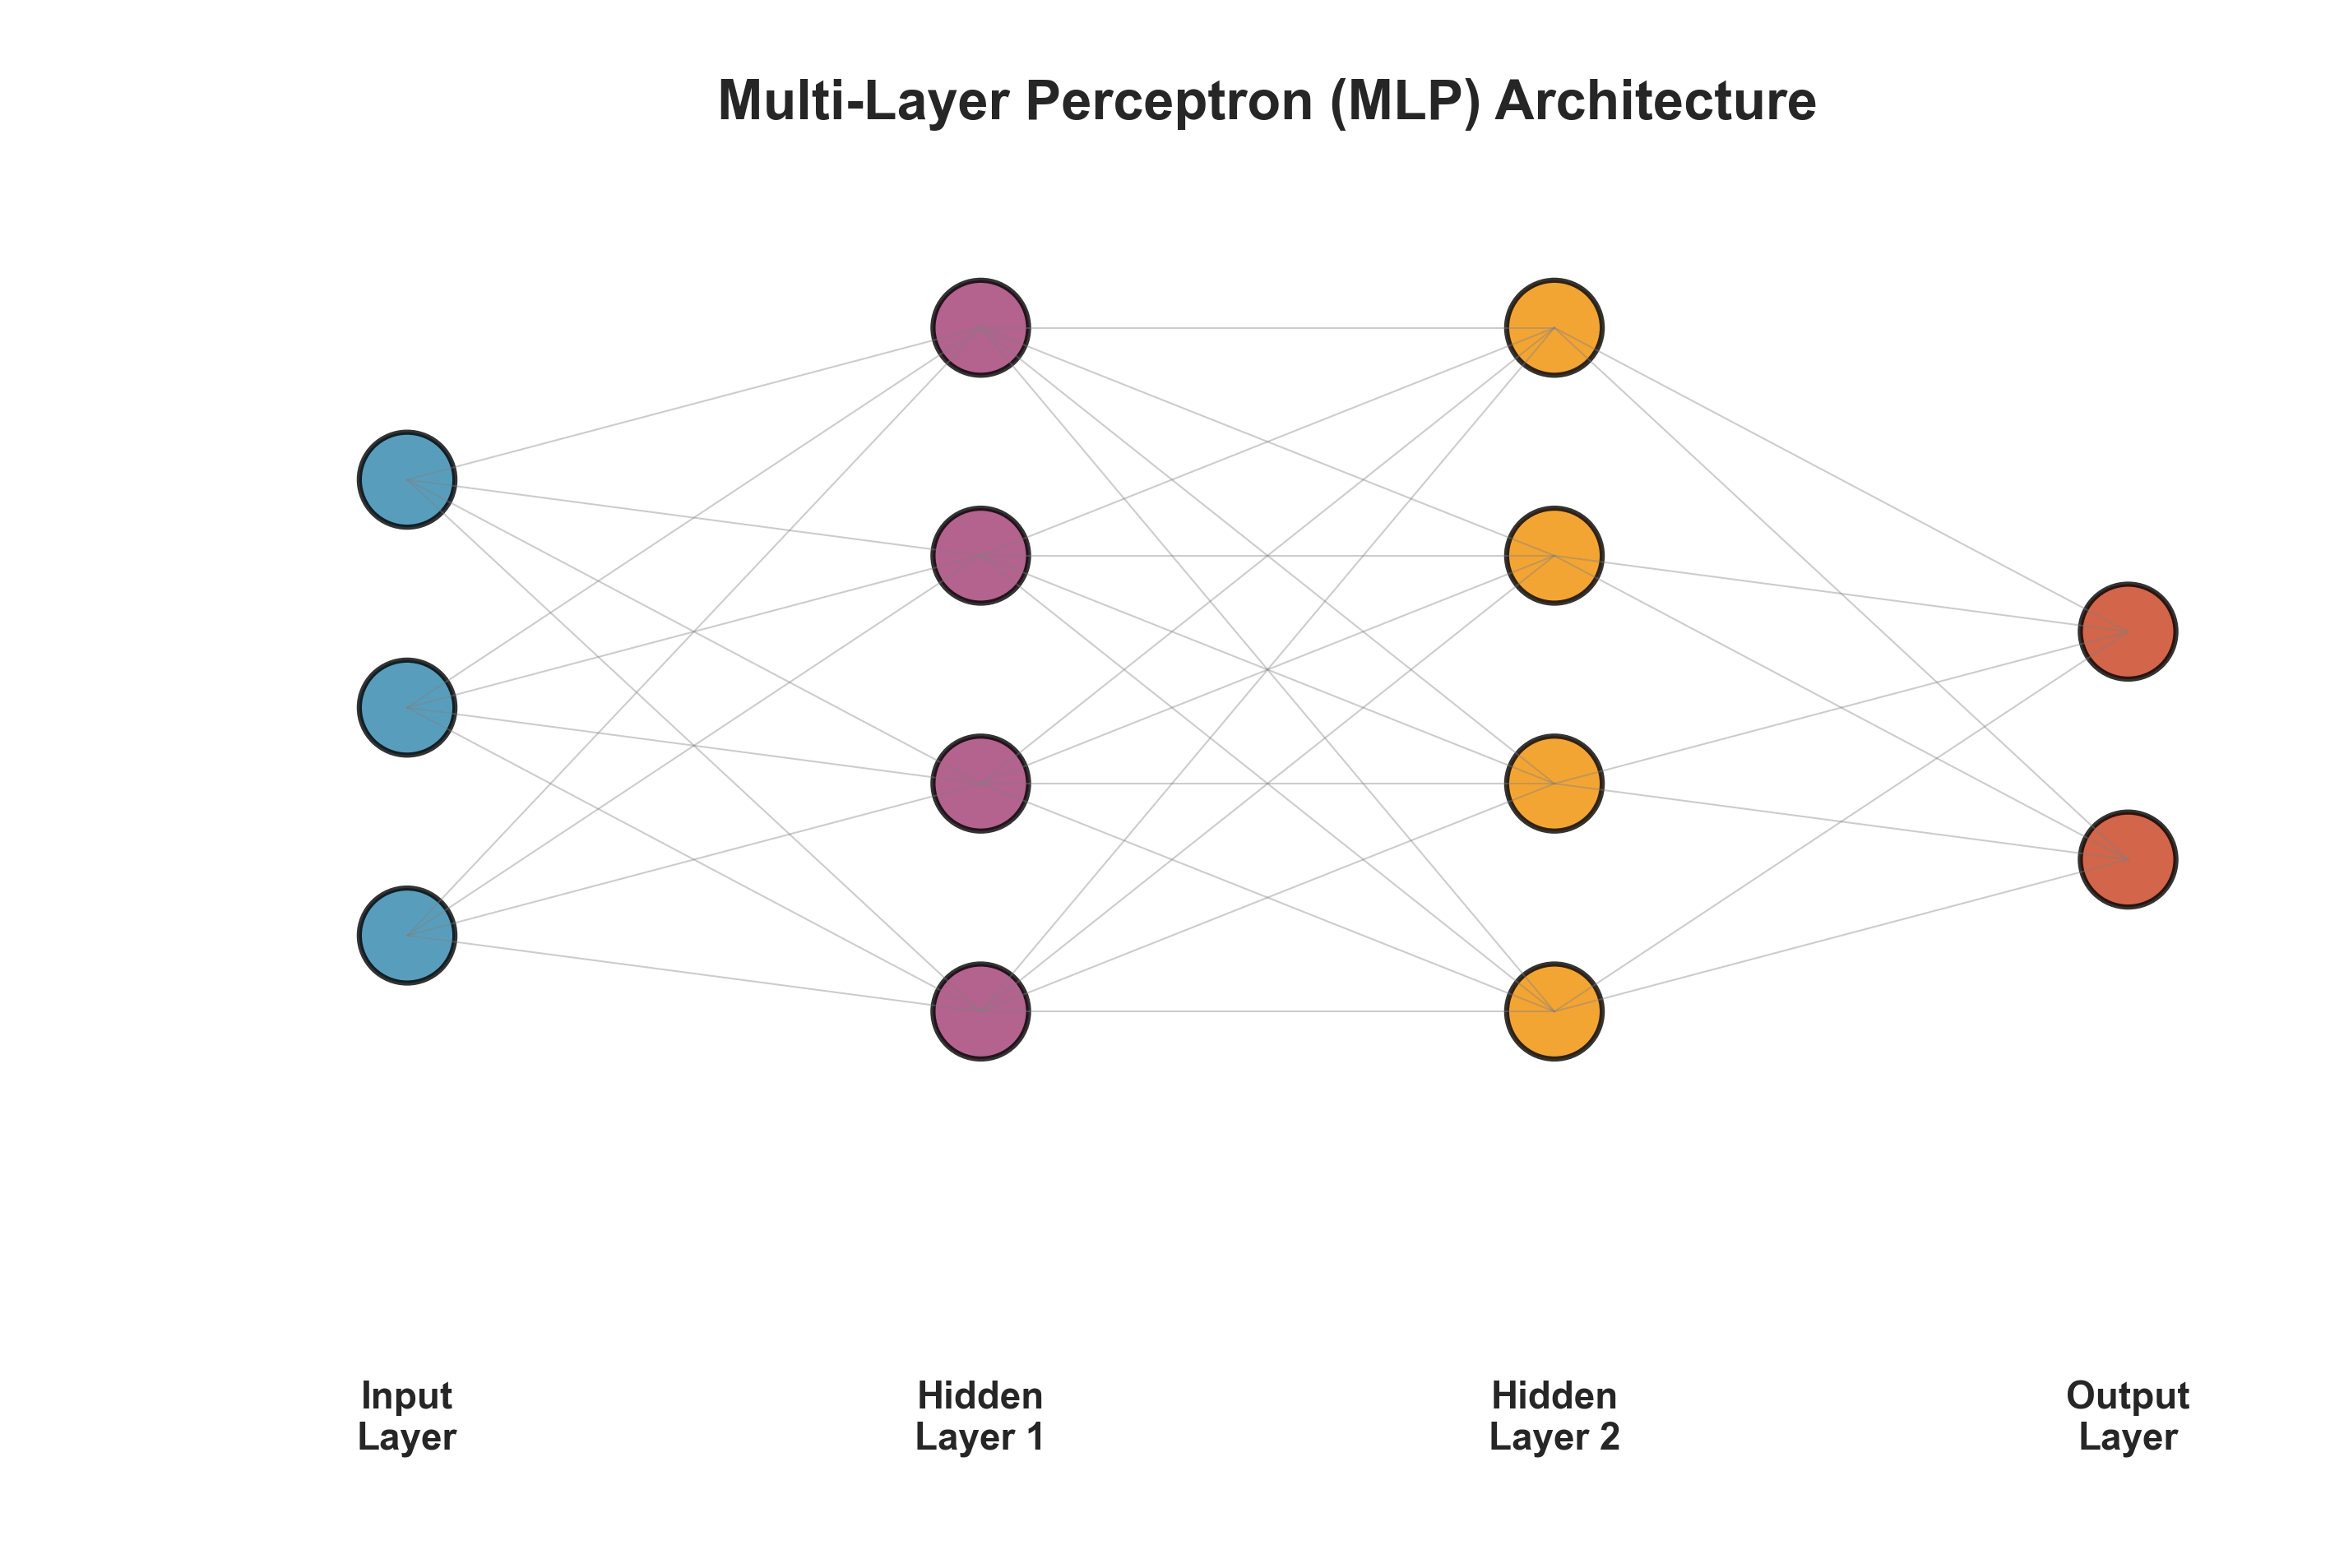
\includegraphics[width=\textwidth]{../figures/03_mlp_architecture.png}\\
\centering{\small Multi-layer perceptron with hidden layers}
\end{columns}
\end{frame}

\begin{frame}{Universal Approximation Theorem}
\begin{alertblock}{Key Theoretical Result}
A feedforward network with a single hidden layer containing a finite number of neurons can approximate any continuous function on compact subsets of $\mathbb{R}^n$, under mild assumptions on the activation function.
\end{alertblock}

\textbf{Implications:}
\begin{itemize}
\item Neural networks are universal function approximators
\item Sufficient network capacity can learn any pattern
\item Depth enables efficient representation
\item More layers = more expressive power
\end{itemize}

\textbf{In Practice:}
\begin{itemize}
\item Deep networks learn hierarchical representations
\item Lower layers capture low-level features
\item Higher layers capture abstract concepts
\end{itemize}
\end{frame}

\section{Activation Functions}

\begin{frame}{Role of Activation Functions}
\begin{alertblock}{Purpose}
Activation functions introduce non-linearity into neural networks, enabling them to learn complex patterns beyond linear transformations.
\end{alertblock}

\textbf{Key Properties:}
\begin{itemize}
\item \textbf{Non-linearity:} Essential for learning complex mappings
\item \textbf{Differentiability:} Required for gradient-based optimization
\item \textbf{Range:} Controls output magnitude
\item \textbf{Monotonicity:} Affects optimization dynamics
\end{itemize}

\textbf{Without Activation Functions:}
$$\mathbf{y} = \mathbf{W}_2(\mathbf{W}_1\mathbf{x}) = (\mathbf{W}_2\mathbf{W}_1)\mathbf{x} = \mathbf{W}\mathbf{x}$$

Multiple layers collapse to a single linear transformation!
\end{frame}

\begin{frame}{Common Activation Functions}
\begin{columns}
\column{0.5\textwidth}
\textbf{Sigmoid:}
$$\sigma(x) = \frac{1}{1 + e^{-x}}$$
\begin{itemize}
\item Range: $(0, 1)$
\item Smooth gradient
\item Prone to saturation
\end{itemize}

\textbf{Hyperbolic Tangent (tanh):}
$$\tanh(x) = \frac{e^x - e^{-x}}{e^x + e^{-x}}$$
\begin{itemize}
\item Range: $(-1, 1)$
\item Zero-centered
\item Also saturates
\end{itemize}

\column{0.45\textwidth}
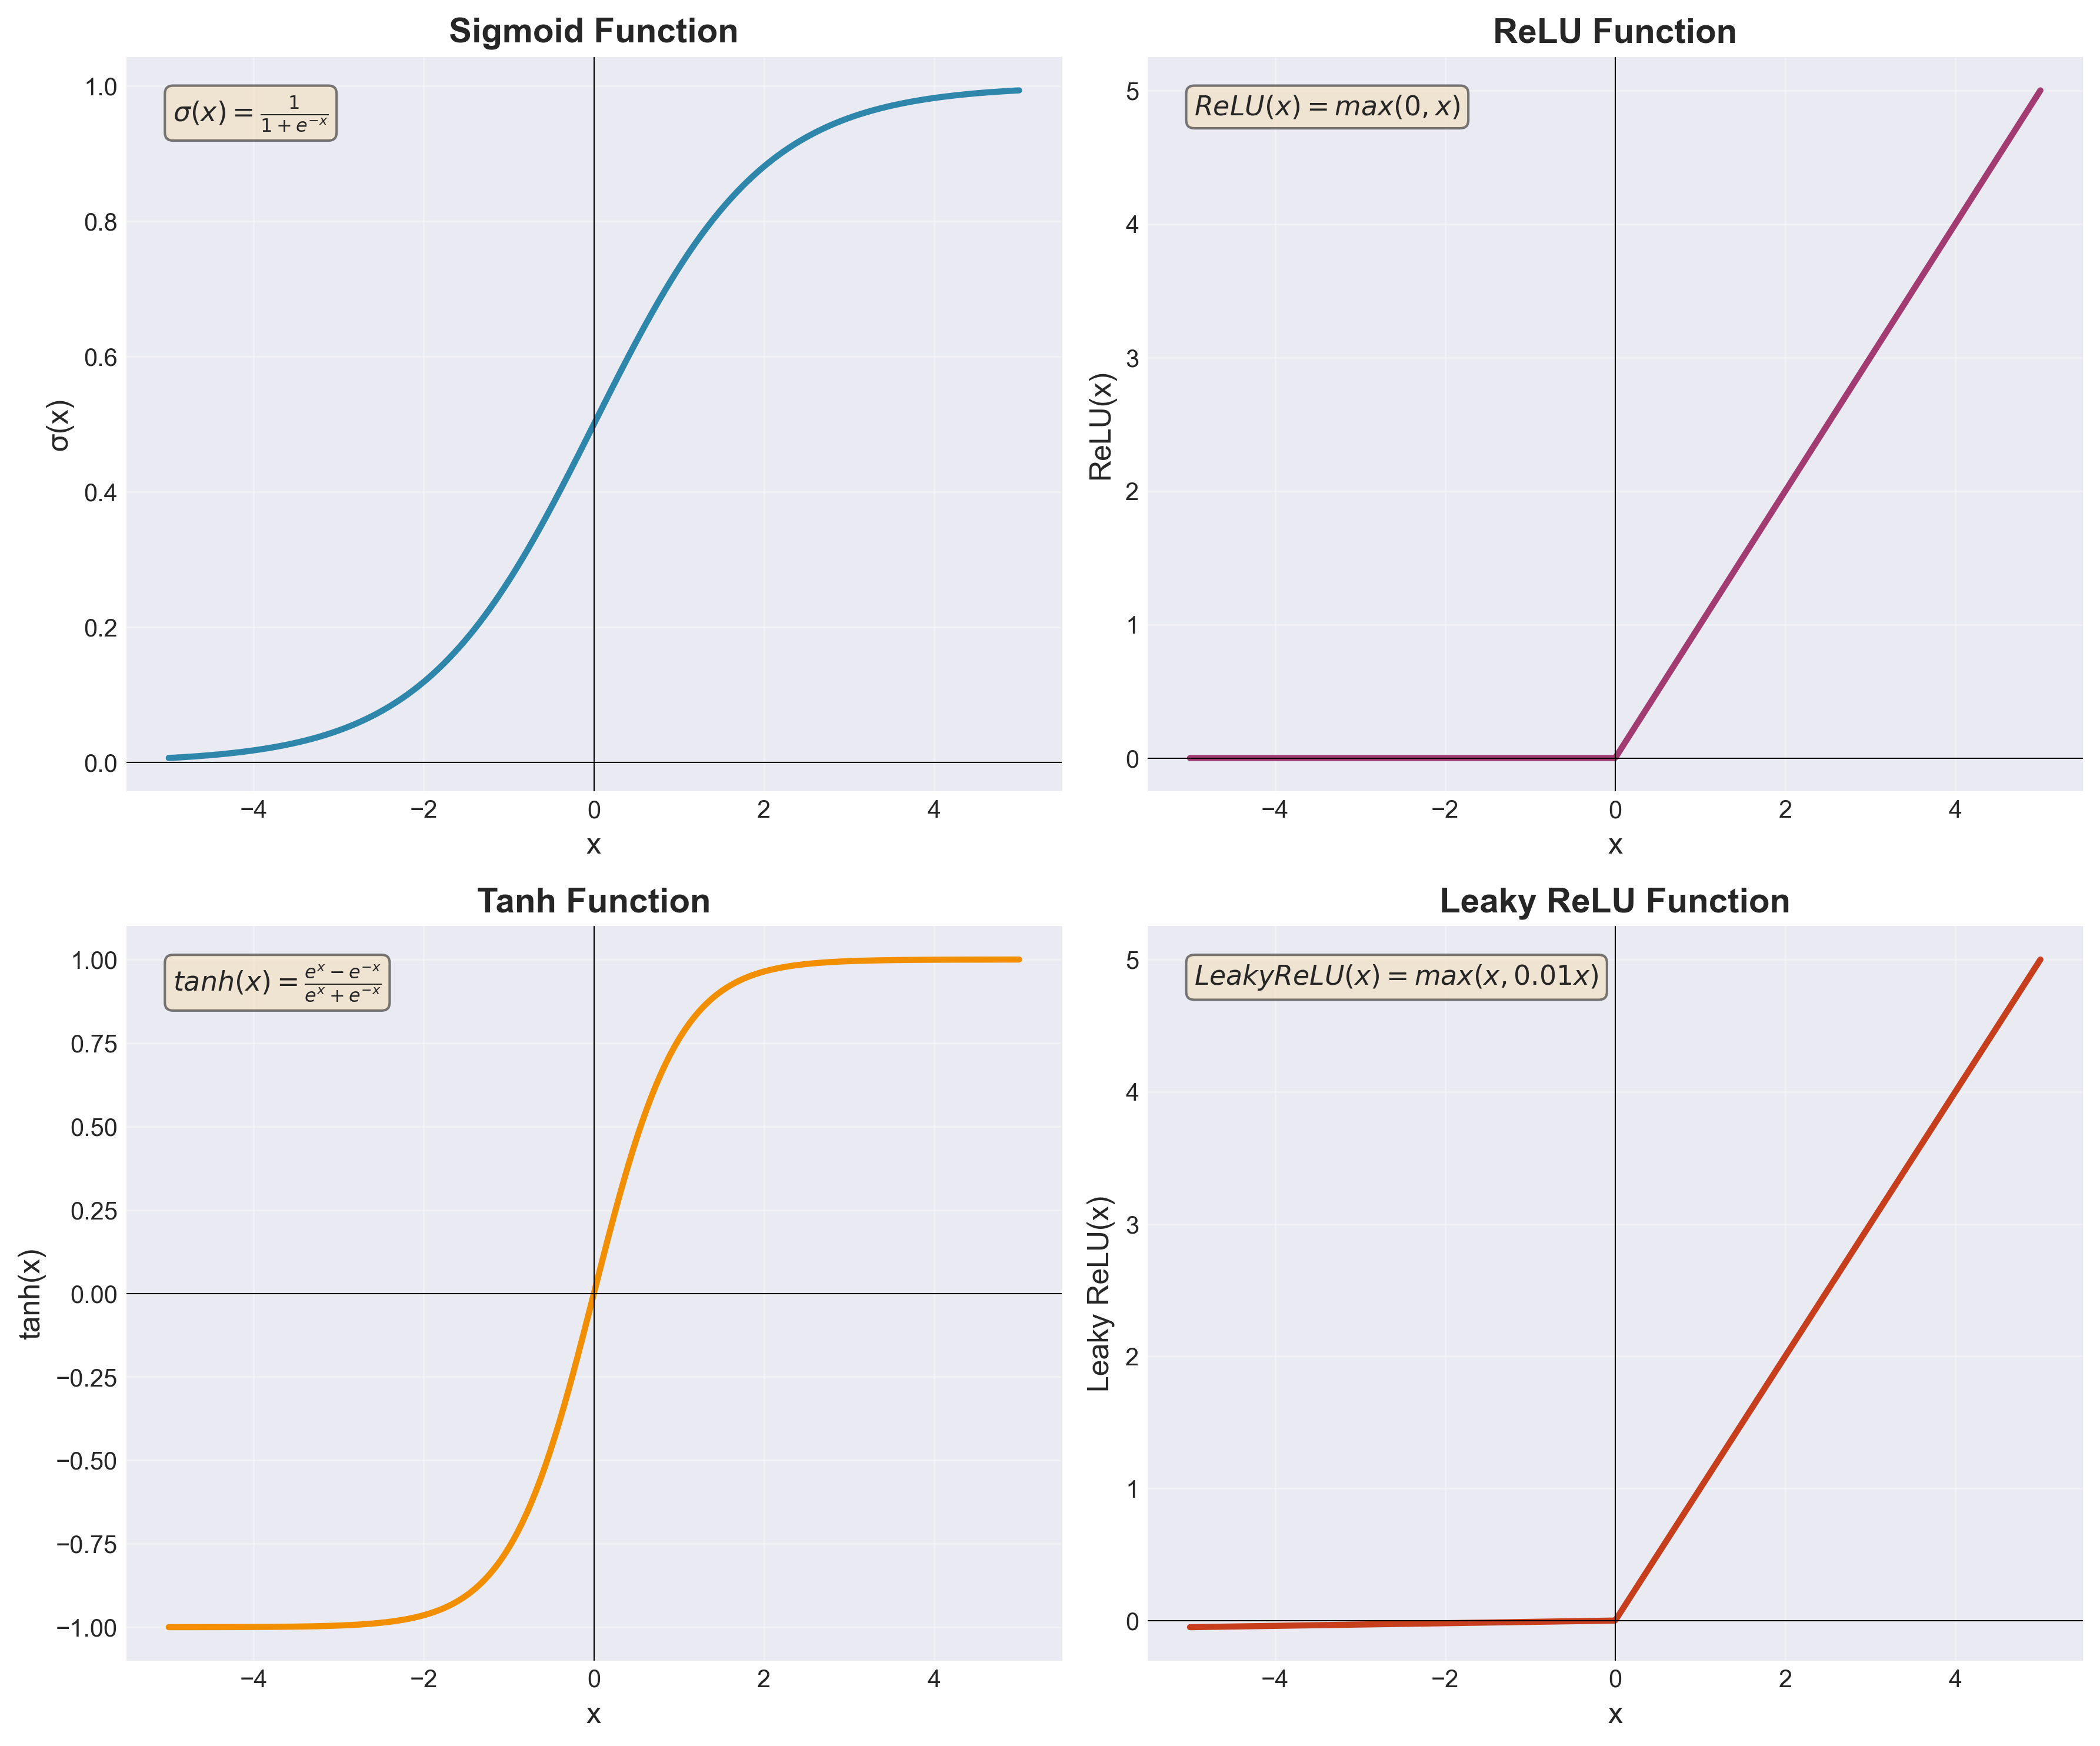
\includegraphics[width=\textwidth]{../figures/01_activation_functions.png}\\
\centering{\small Comparison of activation functions}
\end{columns}
\end{frame}

\begin{frame}{Modern Activation Functions}
\begin{columns}
\column{0.5\textwidth}
\textbf{ReLU (Rectified Linear Unit):}
$$\text{ReLU}(x) = \max(0, x)$$
\begin{itemize}
\item Simple and efficient
\item No saturation for $x > 0$
\item Most popular activation
\end{itemize}

\textbf{Leaky ReLU:}
$$\text{LeakyReLU}(x) = \begin{cases} x & \text{if } x > 0 \\ \alpha x & \text{otherwise} \end{cases}$$
\begin{itemize}
\item Prevents dying neurons
\item Small slope $\alpha \approx 0.01$
\end{itemize}

\column{0.45\textwidth}
\textbf{Advantages of ReLU:}
\begin{enumerate}
\item Computational efficiency
\item Mitigates vanishing gradients
\item Better gradient flow
\end{enumerate}

\textbf{Variants:}
\begin{itemize}
\item \textbf{PReLU:} Learnable $\alpha$
\item \textbf{ELU:} Exponential for $x < 0$
\item \textbf{Swish:} $x \cdot \sigma(x)$
\end{itemize}
\end{columns}
\end{frame}

\section{Loss Functions}

\begin{frame}{Loss Functions in Deep Learning}
\begin{alertblock}{Definition}
A loss function (or cost function) quantifies the difference between predicted outputs and ground truth labels, guiding the optimization process.
\end{alertblock}

\textbf{General Form:}
$$\mathcal{L}(\theta) = \frac{1}{N}\sum_{i=1}^{N} L(y_i, \hat{y}_i) + \lambda R(\theta)$$

Where:
\begin{itemize}
\item $L(\cdot)$ = per-sample loss
\item $y_i$ = ground truth label
\item $\hat{y}_i$ = predicted output
\item $R(\theta)$ = regularization term
\item $\lambda$ = regularization strength
\end{itemize}
\end{frame}

\begin{frame}{Regression Loss Functions}
\begin{columns}
\column{0.5\textwidth}
\textbf{Mean Squared Error (MSE):}
$$\mathcal{L}_{\text{MSE}} = \frac{1}{N}\sum_{i=1}^{N} (y_i - \hat{y}_i)^2$$

\begin{itemize}
\item Differentiable everywhere
\item Sensitive to outliers
\end{itemize}

\textbf{Mean Absolute Error (MAE):}
$$\mathcal{L}_{\text{MAE}} = \frac{1}{N}\sum_{i=1}^{N} |y_i - \hat{y}_i|$$

\begin{itemize}
\item Robust to outliers
\item Linear penalty
\end{itemize}

\column{0.45\textwidth}
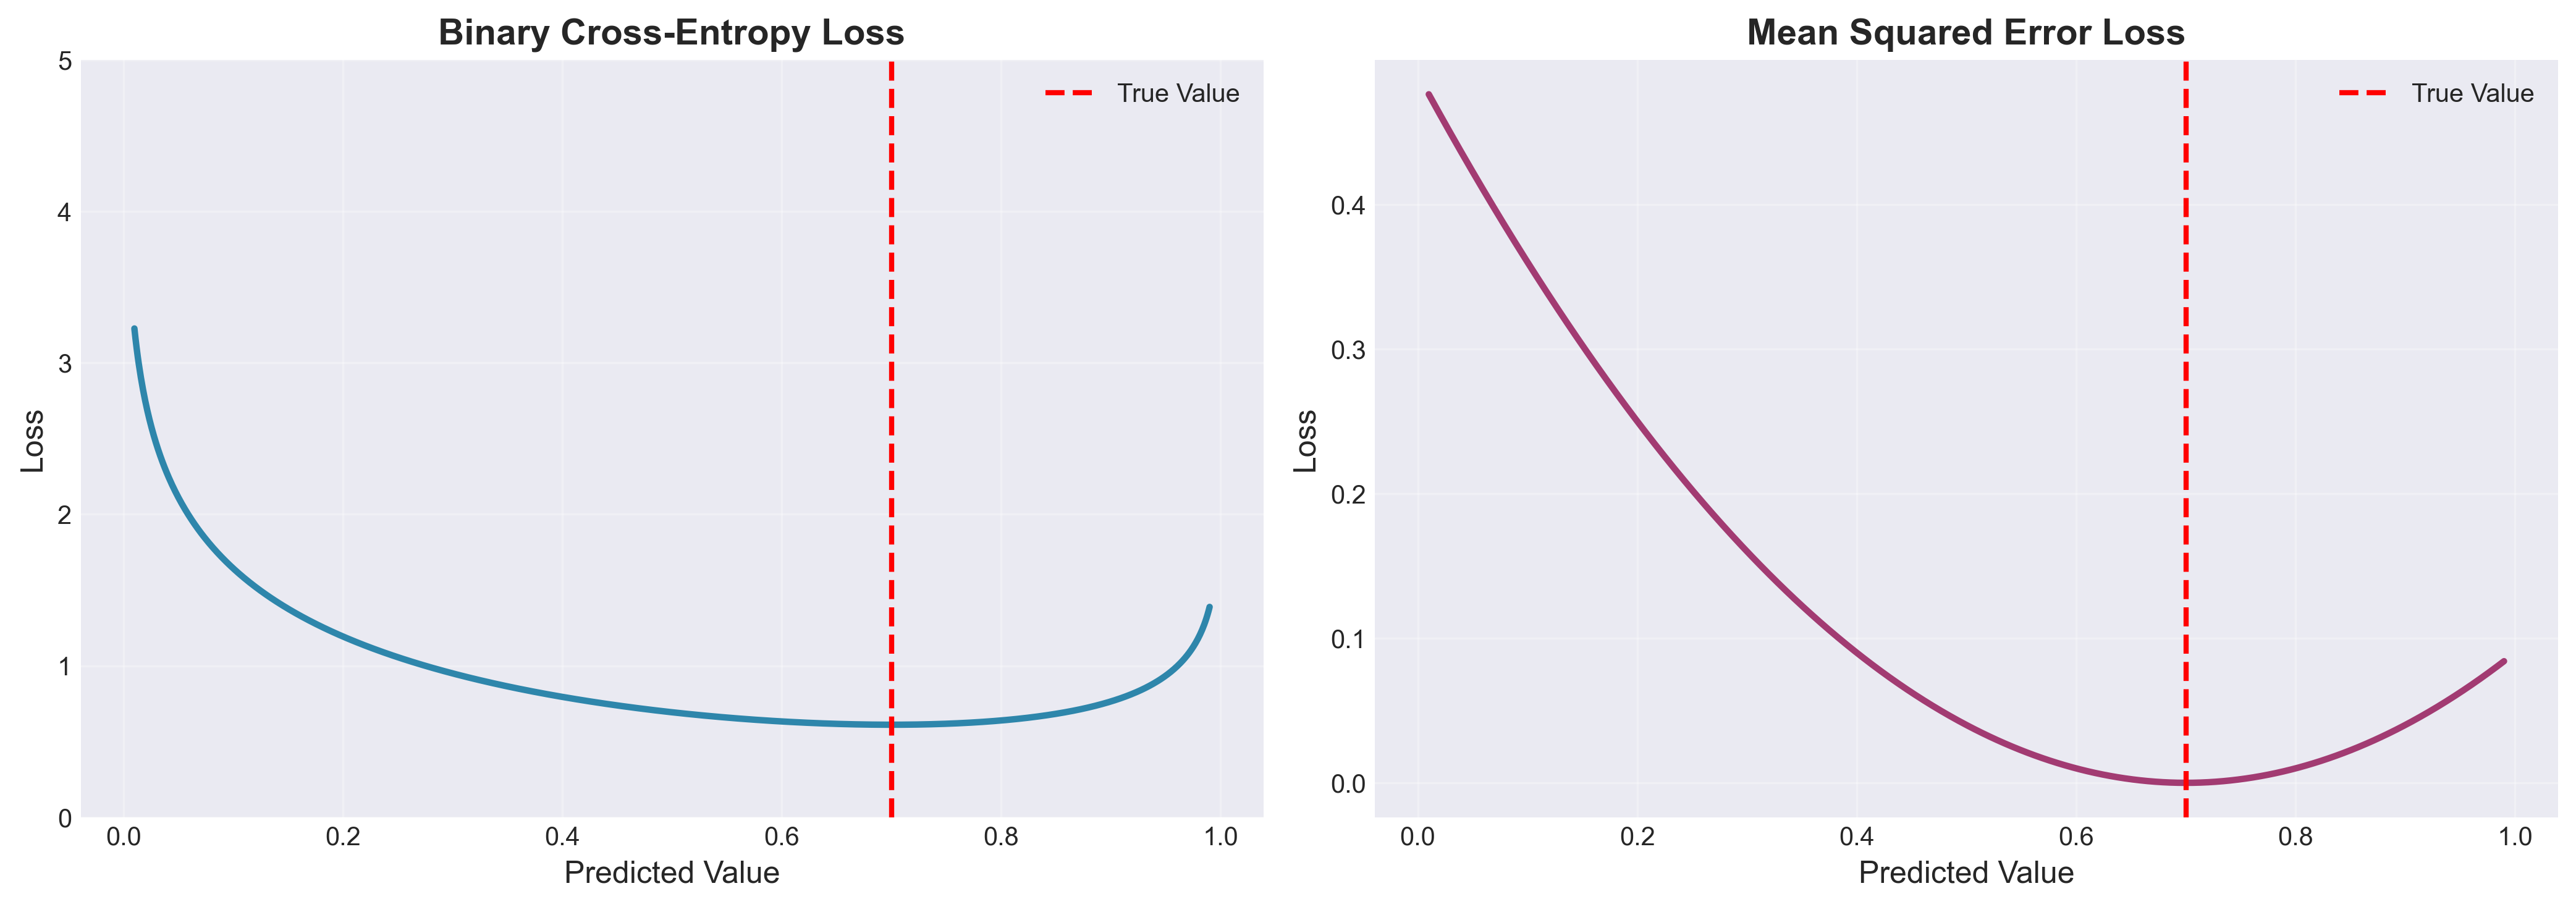
\includegraphics[width=\textwidth]{../figures/04_loss_functions.png}\\
\centering{\small Comparison of different loss functions}
\end{columns}
\end{frame}

\begin{frame}{Classification Loss Functions}
\textbf{Binary Cross-Entropy:}
$$\mathcal{L}_{\text{BCE}} = -\frac{1}{N}\sum_{i=1}^{N} \left[y_i \log(\hat{y}_i) + (1-y_i)\log(1-\hat{y}_i)\right]$$

\textbf{Categorical Cross-Entropy:}
$$\mathcal{L}_{\text{CCE}} = -\frac{1}{N}\sum_{i=1}^{N}\sum_{c=1}^{C} y_{i,c} \log(\hat{y}_{i,c})$$

Where: $C$ = number of classes, $y_{i,c}$ = 1 if sample $i$ is class $c$, $\hat{y}_{i,c}$ = predicted probability

\begin{alertblock}{Softmax Output}
For multi-class: $\hat{y}_c = \frac{e^{z_c}}{\sum_{j=1}^{C} e^{z_j}}$
\end{alertblock}
\end{frame}

\section{Gradient Descent and Optimization}

\begin{frame}{Gradient Descent Fundamentals}
\begin{columns}
\column{0.5\textwidth}
\textbf{Basic Principle:}
$$\theta_{t+1} = \theta_t - \eta \nabla_\theta \mathcal{L}(\theta_t)$$

Where:
\begin{itemize}
\item $\theta$ = model parameters
\item $\eta$ = learning rate
\item $\nabla_\theta \mathcal{L}$ = gradient of loss
\end{itemize}

\textbf{Variants:}
\begin{itemize}
\item \textbf{Batch GD:} Full dataset
\item \textbf{Stochastic GD:} Single sample
\item \textbf{Mini-batch GD:} Batch of samples
\end{itemize}

\column{0.45\textwidth}
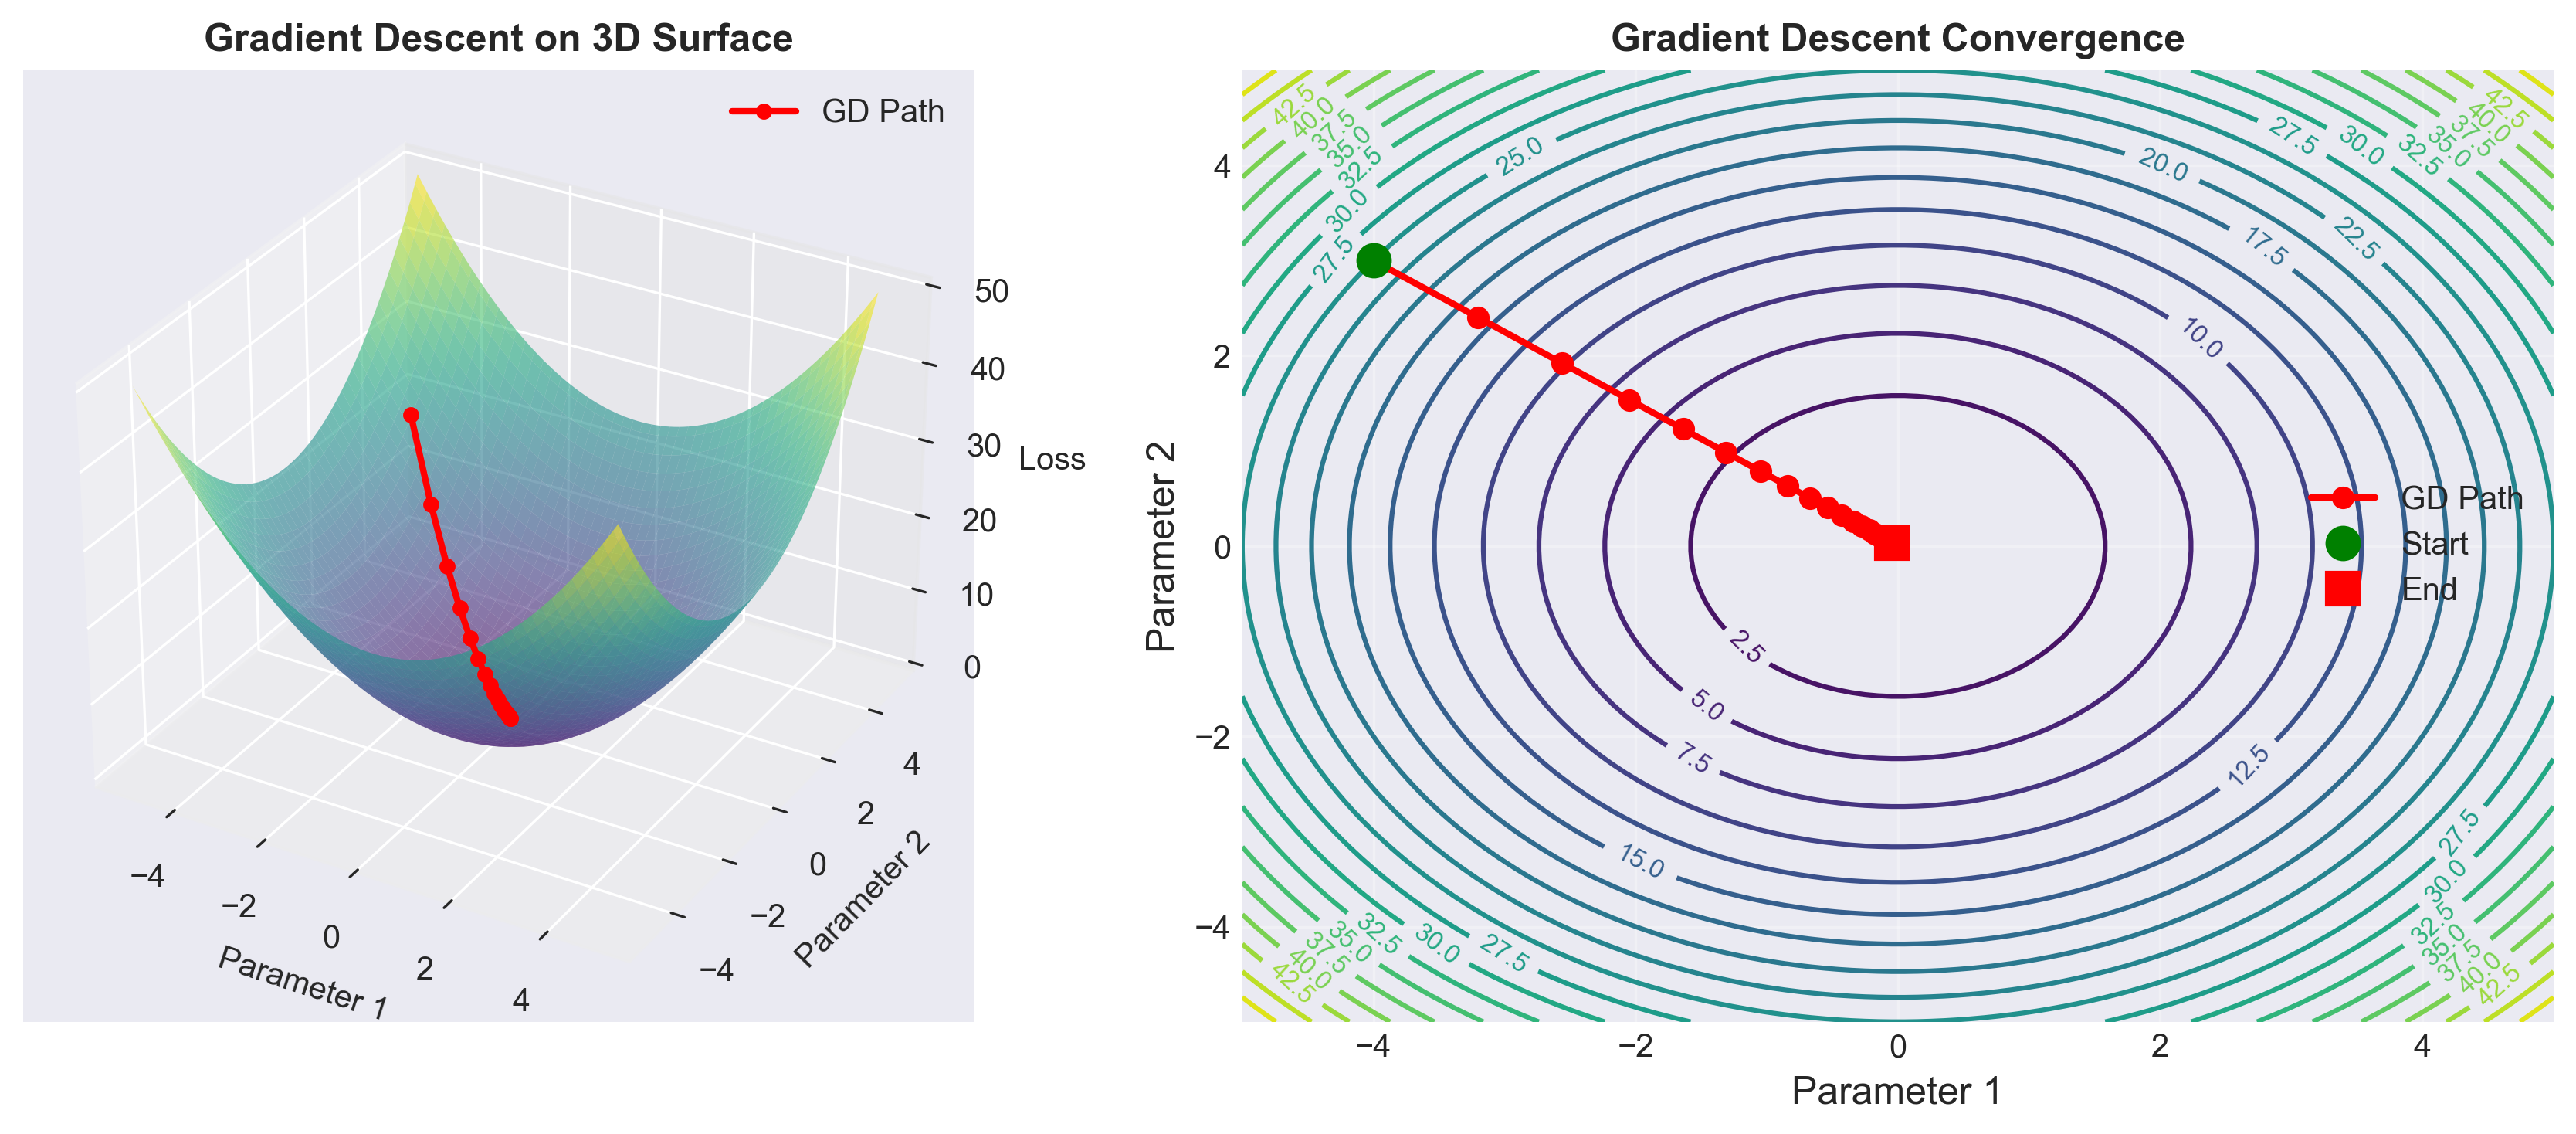
\includegraphics[width=\textwidth]{../figures/05_gradient_descent.png}\\
\centering{\small Gradient descent optimization trajectory}
\end{columns}
\end{frame}

\begin{frame}{Advanced Optimizers}
\begin{columns}
\column{0.5\textwidth}
\textbf{Momentum:}
$$\mathbf{v}_t = \beta \mathbf{v}_{t-1} + \nabla_\theta \mathcal{L}(\theta_t)$$
$$\theta_{t+1} = \theta_t - \eta \mathbf{v}_t$$

\textbf{Adam (Adaptive Moment):}
\begin{align}
\mathbf{m}_t &= \beta_1 \mathbf{m}_{t-1} + (1-\beta_1)\mathbf{g}_t \\
\mathbf{v}_t &= \beta_2 \mathbf{v}_{t-1} + (1-\beta_2)\mathbf{g}_t^2 \\
\theta_{t+1} &= \theta_t - \eta \frac{\hat{\mathbf{m}}_t}{\sqrt{\hat{\mathbf{v}}_t} + \epsilon}
\end{align}

\column{0.45\textwidth}
\textbf{Optimizer Comparison:}
\begin{itemize}
\item \textbf{SGD:} Simple, requires tuning
\item \textbf{Momentum:} Faster convergence
\item \textbf{RMSprop:} Adaptive learning rates
\item \textbf{Adam:} Combines best of both
\end{itemize}

\textbf{Hyperparameters:}
\begin{itemize}
\item Learning rate: $\eta$
\item Momentum: $\beta \approx 0.9$
\item Adam: $\beta_1=0.9, \beta_2=0.999$
\end{itemize}
\end{columns}
\end{frame}

\begin{frame}{Learning Rate Scheduling}
\textbf{Why Schedule Learning Rates?}
\begin{itemize}
\item Start with large steps for fast initial progress
\item Reduce step size for fine-tuning near optimum
\item Prevent oscillations and divergence
\end{itemize}

\textbf{Common Schedules:}

\textbf{Step Decay:}
$$\eta_t = \eta_0 \cdot \gamma^{\lfloor t/s \rfloor}$$

\textbf{Exponential Decay:}
$$\eta_t = \eta_0 \cdot e^{-\lambda t}$$

\textbf{Cosine Annealing:}
$$\eta_t = \eta_{\min} + \frac{1}{2}(\eta_{\max} - \eta_{\min})\left(1 + \cos\left(\frac{t\pi}{T}\right)\right)$$
\end{frame}

\section{Backpropagation}

\begin{frame}{Backpropagation Algorithm}
\begin{alertblock}{Core Principle}
Backpropagation efficiently computes gradients of the loss function with respect to all network parameters using the chain rule of calculus.
\end{alertblock}

\textbf{Chain Rule:}
$$\frac{\partial \mathcal{L}}{\partial w_i} = \frac{\partial \mathcal{L}}{\partial y} \cdot \frac{\partial y}{\partial z} \cdot \frac{\partial z}{\partial w_i}$$

\textbf{Algorithm Steps:}
\begin{enumerate}
\item \textbf{Forward pass:} Compute activations and outputs
\item \textbf{Compute loss:} Evaluate error at output
\item \textbf{Backward pass:} Propagate gradients from output to input
\item \textbf{Update weights:} Apply gradient descent
\end{enumerate}
\end{frame}

\begin{frame}{Backpropagation Mathematics}
\textbf{For a single layer:}
$$z^{(l)} = W^{(l)}a^{(l-1)} + b^{(l)}$$
$$a^{(l)} = f(z^{(l)})$$

\textbf{Gradient computation:}
$$\delta^{(l)} = \frac{\partial \mathcal{L}}{\partial z^{(l)}} = \frac{\partial \mathcal{L}}{\partial a^{(l)}} \odot f'(z^{(l)})$$

\textbf{Weight gradients:}
$$\frac{\partial \mathcal{L}}{\partial W^{(l)}} = \delta^{(l)} (a^{(l-1)})^T$$

\textbf{Recursive gradient:}
$$\delta^{(l-1)} = (W^{(l)})^T \delta^{(l)} \odot f'(z^{(l-1)})$$
\end{frame}

\begin{frame}{Computational Efficiency}
\begin{columns}
\column{0.5\textwidth}
\textbf{Why Backpropagation?}

\textbf{Naive approach:}
\begin{itemize}
\item Compute each gradient independently
\item Complexity: $O(n \cdot m)$ where $n$ = parameters, $m$ = samples
\item Redundant computations
\end{itemize}

\textbf{Backpropagation:}
\begin{itemize}
\item Reuse intermediate results
\item Complexity: $O(m)$
\item Single backward pass
\item Memory-efficient
\end{itemize}

\column{0.45\textwidth}
\textbf{Gradient Flow:}
\begin{itemize}
\item Forward: Input → Output
\item Backward: Output → Input
\item Automatic differentiation
\item Modern frameworks handle this
\end{itemize}

\textbf{Challenges:}
\begin{itemize}
\item Vanishing gradients
\item Exploding gradients
\item Dead neurons
\end{itemize}
\end{columns}
\end{frame}

\section{Convolutional Neural Networks}

\begin{frame}{Introduction to CNNs}
\begin{alertblock}{Key Insight}
Convolutional Neural Networks leverage spatial structure in images through parameter sharing and local connectivity, dramatically reducing parameters while improving performance.
\end{alertblock}

\textbf{Motivation for CNNs:}
\begin{itemize}
\item Images have spatial structure (nearby pixels are correlated)
\item Fully-connected networks ignore this structure
\item Too many parameters for high-resolution images
\item Translation invariance is desirable
\end{itemize}

\textbf{CNN Principles:}
\begin{itemize}
\item \textbf{Local connectivity:} Each neuron sees only local region
\item \textbf{Parameter sharing:} Same weights across spatial locations
\item \textbf{Hierarchical features:} Low to high-level representations
\end{itemize}
\end{frame}

\begin{frame}{CNN Architecture Overview}
\begin{columns}
\column{0.5\textwidth}
\textbf{Typical CNN Layers:}
\begin{enumerate}
\item \textbf{Convolution:} Feature extraction
\item \textbf{Activation:} Non-linearity (ReLU)
\item \textbf{Pooling:} Spatial downsampling
\item \textbf{Fully-connected:} Classification
\end{enumerate}

\textbf{Information Flow:}
\small
$$\text{Input} \rightarrow \text{Conv} \rightarrow \text{ReLU} \rightarrow \text{Pool} \rightarrow \cdots \rightarrow \text{FC}$$

\column{0.45\textwidth}
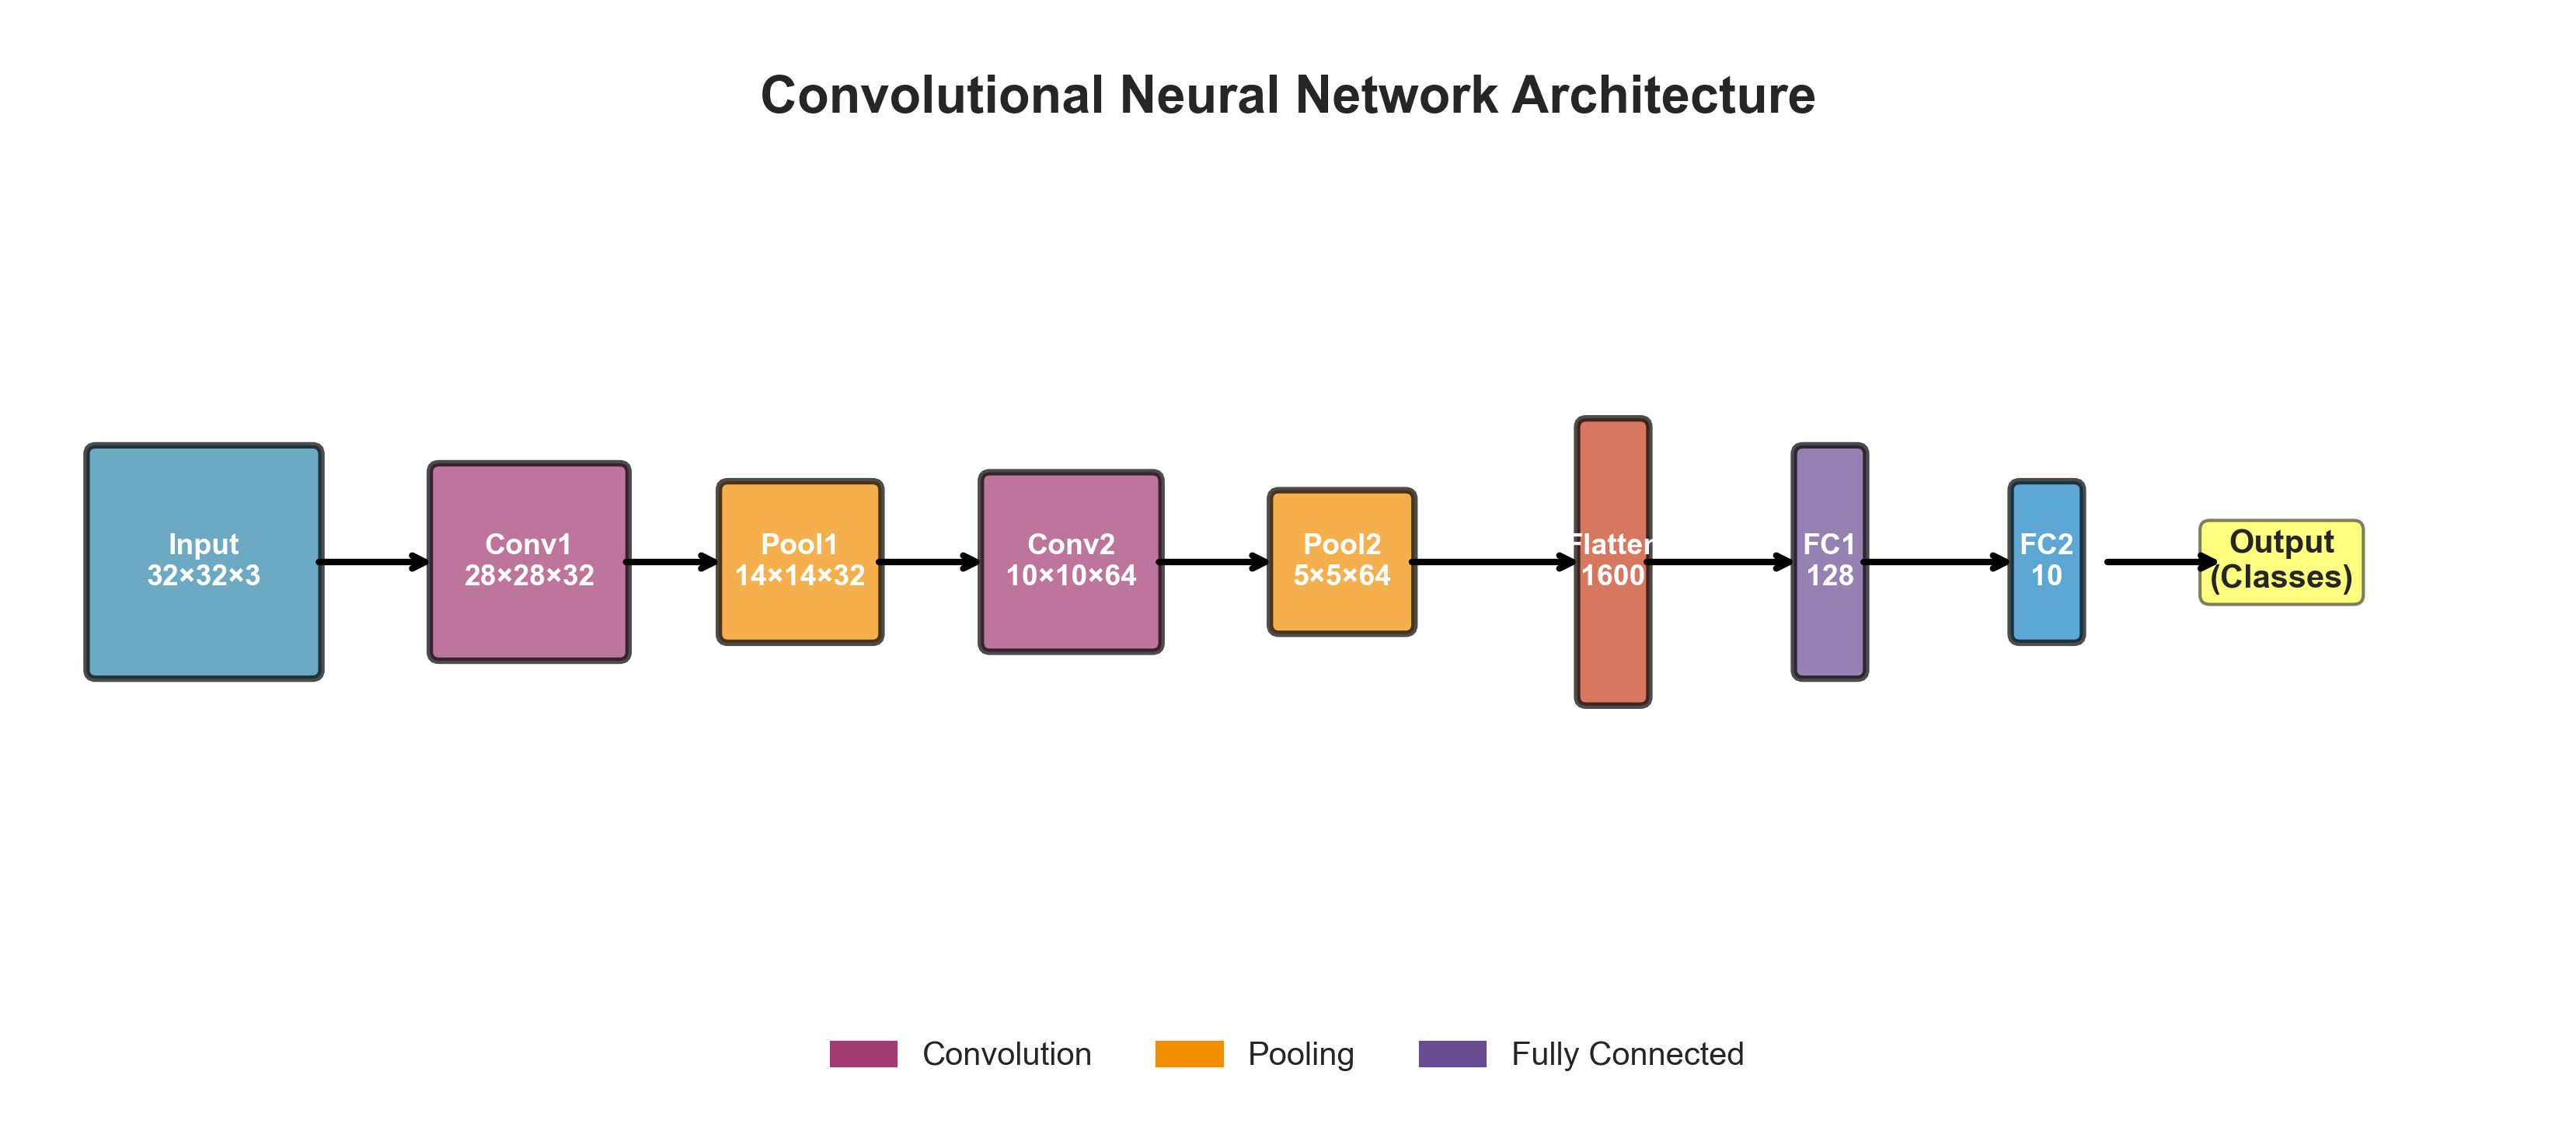
\includegraphics[width=\textwidth]{../figures/08_cnn_architecture.png}\\
\centering{\small Complete CNN architecture}
\end{columns}
\end{frame}

\begin{frame}{Convolution Operation}
\begin{columns}
\column{0.5\textwidth}
\textbf{2D Convolution:}
$$Y[i,j] = \sum_{m}\sum_{n} X[i+m, j+n] \cdot K[m,n]$$

Where:
\begin{itemize}
\item $X$ = input feature map
\item $K$ = convolution kernel/filter
\item $Y$ = output feature map
\end{itemize}

\textbf{Key Parameters:}
\begin{itemize}
\item \textbf{Kernel size:} $k \times k$ (e.g., 3×3, 5×5)
\item \textbf{Stride:} Step size ($s$)
\item \textbf{Padding:} Border handling
\end{itemize}

\column{0.45\textwidth}
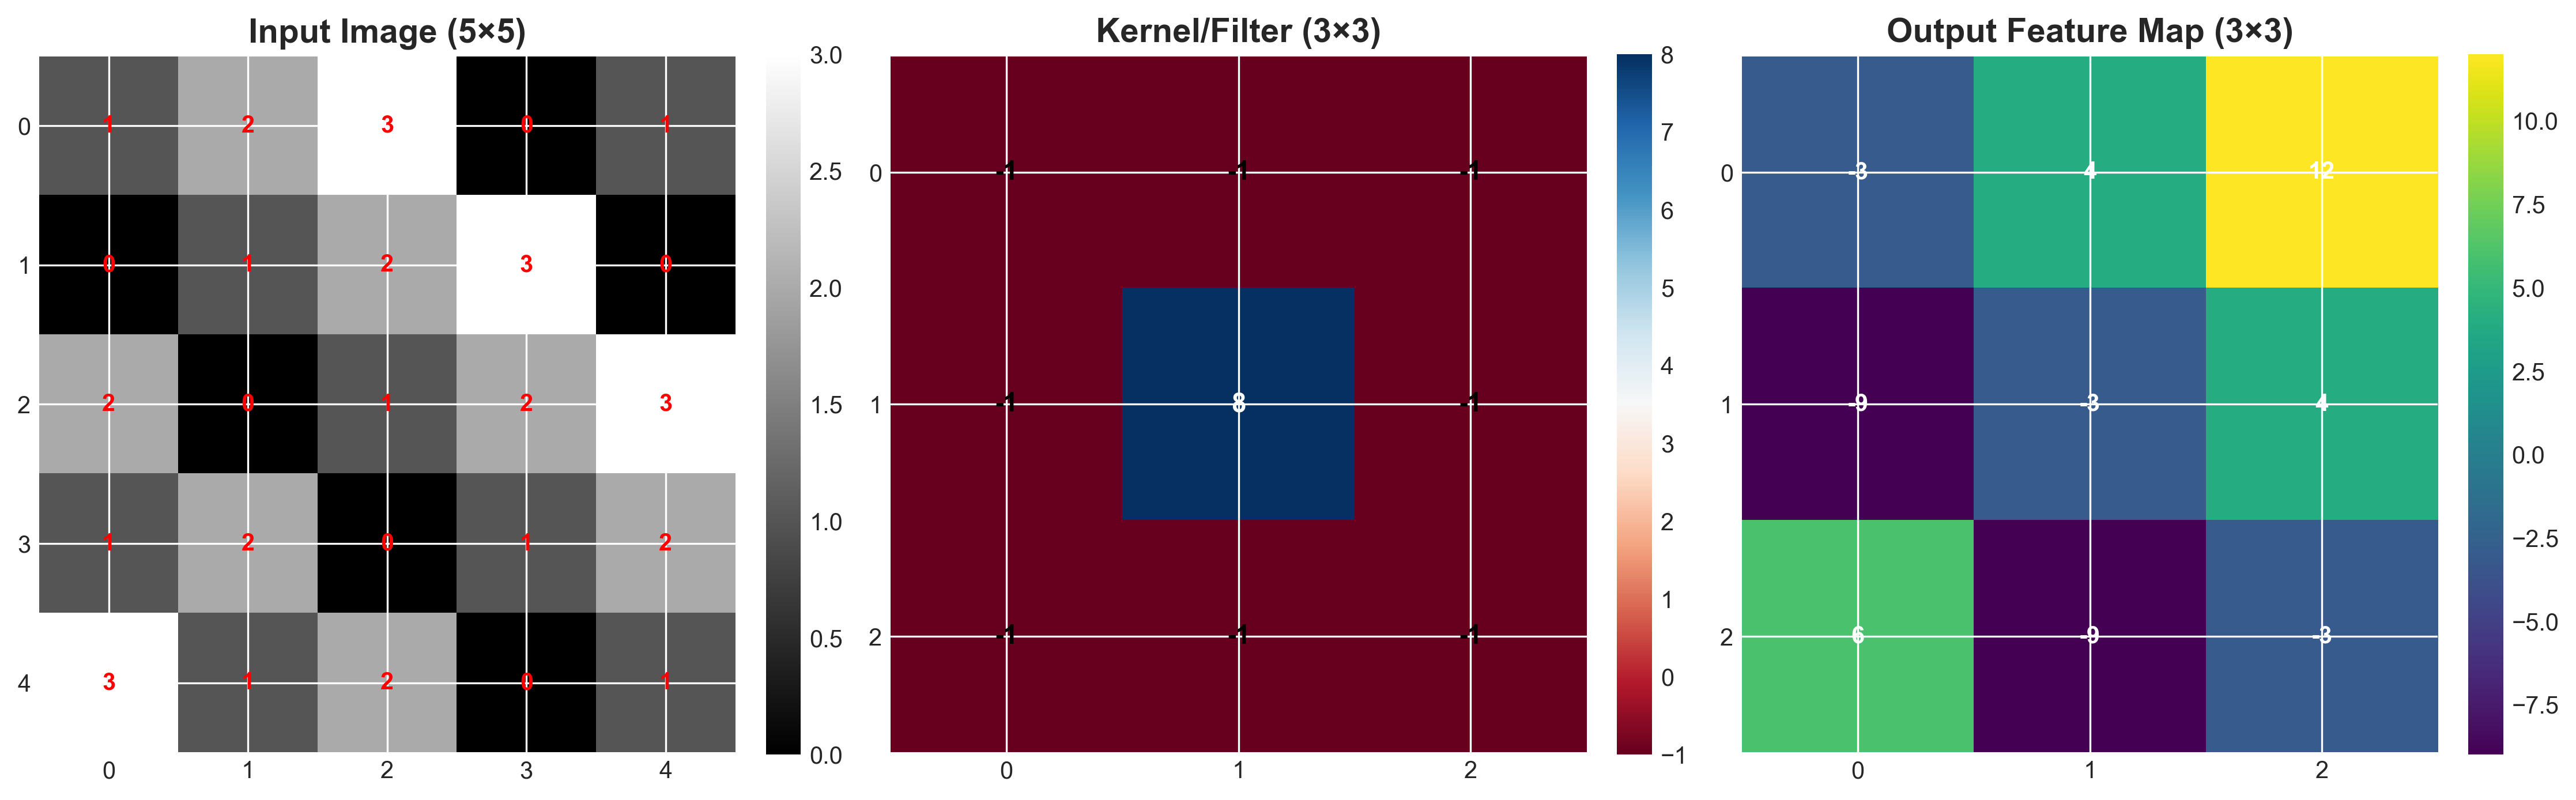
\includegraphics[width=\textwidth]{../figures/06_convolution_operation.png}\\
\centering{\small Convolution operation with kernel sliding over input}
\end{columns}
\end{frame}

\begin{frame}{Convolution Mathematics}
\textbf{Output Dimensions:}
$$H_{\text{out}} = \left\lfloor \frac{H_{\text{in}} + 2p - k}{s} \right\rfloor + 1$$
$$W_{\text{out}} = \left\lfloor \frac{W_{\text{in}} + 2p - k}{s} \right\rfloor + 1$$

Where:
\begin{itemize}
\item $H, W$ = height, width
\item $p$ = padding
\item $k$ = kernel size
\item $s$ = stride
\end{itemize}

\textbf{Padding Types:}
\begin{itemize}
\item \textbf{Valid:} No padding ($p=0$), output size decreases
\item \textbf{Same:} $p = \lfloor k/2 \rfloor$, output size preserved (for $s=1$)
\end{itemize}
\end{frame}

\begin{frame}{Feature Maps and Filters}
\begin{columns}
\column{0.5\textwidth}
\textbf{Multiple Channels:}
$$Y_k = \sum_{c=1}^{C_{\text{in}}} X_c \star K_{k,c} + b_k$$

\textbf{Parameters:}
\begin{itemize}
\item Input: $H \times W \times C_{\text{in}}$
\item Kernel: $k \times k \times C_{\text{in}} \times C_{\text{out}}$
\item Output: $H' \times W' \times C_{\text{out}}$
\end{itemize}

\textbf{Number of Parameters:}
$$\text{Params} = k^2 \cdot C_{\text{in}} \cdot C_{\text{out}} + C_{\text{out}}$$

\column{0.45\textwidth}
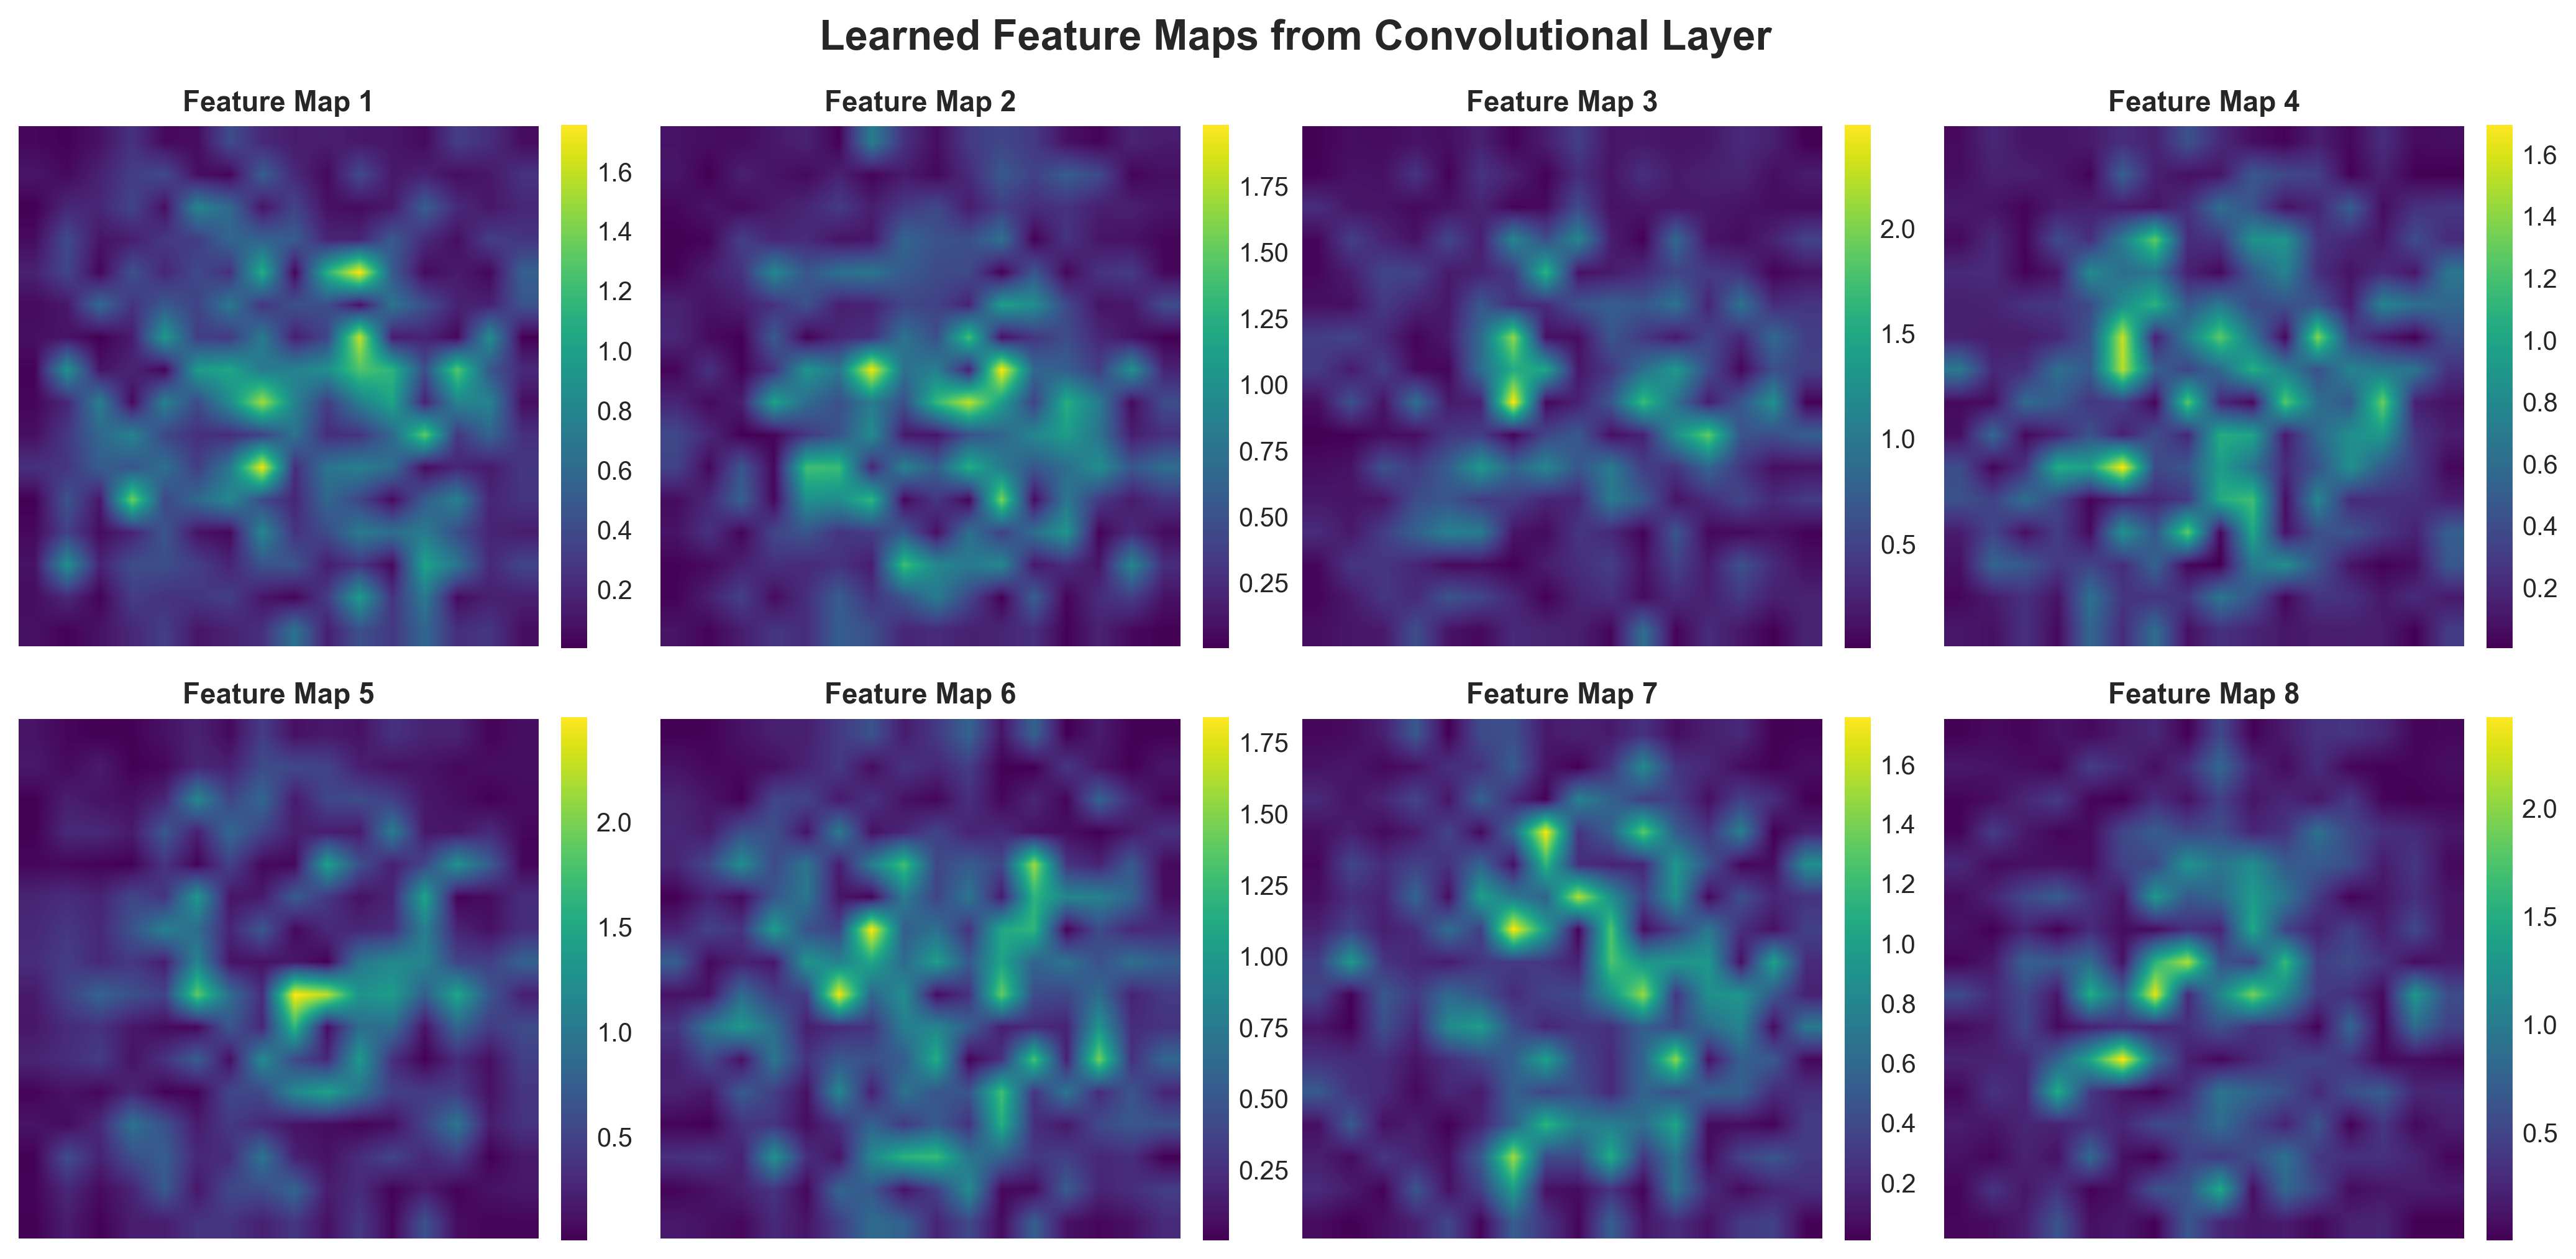
\includegraphics[width=\textwidth]{../figures/09_feature_maps.png}\\
\centering{\small Feature maps at different network depths}
\end{columns}
\end{frame}

\section{Pooling Layers}

\begin{frame}{Pooling Operations}
\begin{columns}
\column{0.5\textwidth}
\begin{alertblock}{Purpose of Pooling}
Pooling reduces spatial dimensions while retaining important features, providing translation invariance and computational efficiency.
\end{alertblock}

\textbf{Max Pooling:}
$$Y[i,j] = \max_{m,n \in \mathcal{R}_{i,j}} X[m,n]$$

\textbf{Average Pooling:}
$$Y[i,j] = \frac{1}{|\mathcal{R}_{i,j}|} \sum_{m,n \in \mathcal{R}_{i,j}} X[m,n]$$

\column{0.45\textwidth}
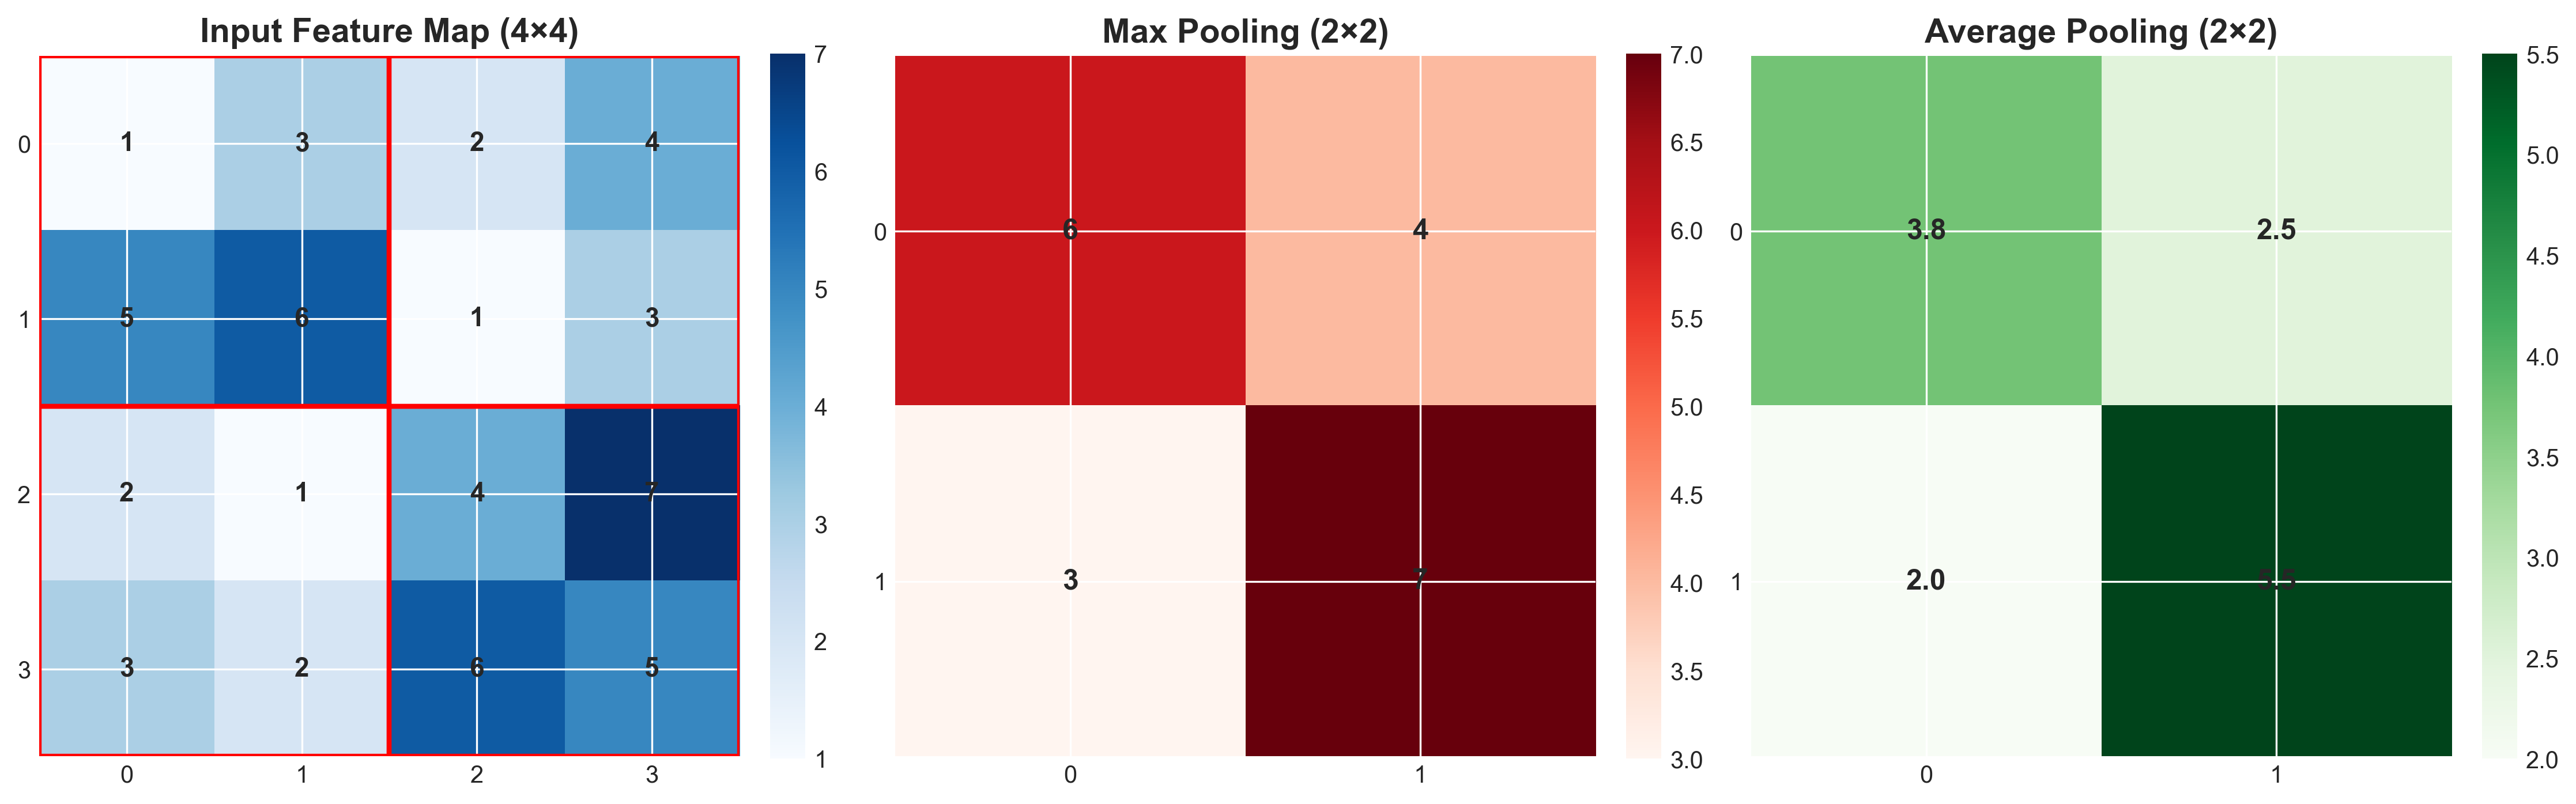
\includegraphics[width=\textwidth]{../figures/07_pooling_operations.png}\\
\centering{\small Max and average pooling operations}
\end{columns}
\end{frame}

\begin{frame}{Pooling Properties}
\textbf{Advantages:}
\begin{itemize}
\item \textbf{Dimensionality reduction:} Reduces computation
\item \textbf{Translation invariance:} Tolerates small shifts
\item \textbf{Feature selection:} Max pooling keeps strongest activations
\item \textbf{No parameters:} No learning required
\end{itemize}

\textbf{Common Configurations:}
\begin{itemize}
\item $2 \times 2$ window with stride 2 (most common)
\item $3 \times 3$ window with stride 2
\item Global average/max pooling (reduces to 1×1)
\end{itemize}

\textbf{Trends:}
\begin{itemize}
\item Modern architectures often use strided convolutions instead
\item Global pooling popular for final feature aggregation
\end{itemize}
\end{frame}

\section{CNN Architectures}

\begin{frame}{Classic CNN Architectures}
\textbf{LeNet-5 (1998):}
\begin{itemize}
\item First successful CNN for digit recognition
\item Conv → Pool → Conv → Pool → FC → FC
\end{itemize}

\textbf{AlexNet (2012):}
\begin{itemize}
\item ImageNet breakthrough
\item 5 conv layers, 3 FC layers, ReLU, dropout
\end{itemize}

\textbf{VGGNet (2014):}
\begin{itemize}
\item Very deep (16-19 layers)
\item Small 3×3 filters, simple architecture
\end{itemize}

\textbf{Key Insight:} Deeper networks with smaller filters outperform shallow networks.
\end{frame}

\begin{frame}{Modern CNN Architectures}
\textbf{ResNet (2015):}
\begin{itemize}
\item Residual connections: $y = f(x) + x$
\item Enables training very deep networks (50-152 layers)
\item Solves vanishing gradient problem
\end{itemize}

\textbf{Inception/GoogLeNet (2014):}
\begin{itemize}
\item Multi-scale feature extraction
\item Inception modules with parallel paths
\item Efficient parameter usage
\end{itemize}

\textbf{EfficientNet (2019):}
\begin{itemize}
\item Compound scaling (depth, width, resolution)
\item State-of-the-art efficiency
\item Neural architecture search
\end{itemize}
\end{frame}

\section{Training Deep Networks}

\begin{frame}{Training Pipeline}
\begin{columns}
\column{0.5\textwidth}
\textbf{Complete Training Loop:}
\begin{enumerate}
\item \textbf{Data loading:} Load mini-batch
\item \textbf{Forward pass:} Compute predictions
\item \textbf{Loss computation:} Calculate error
\item \textbf{Backward pass:} Compute gradients
\item \textbf{Parameter update:} Apply optimizer
\item \textbf{Evaluation:} Monitor metrics
\end{enumerate}

\textbf{Hyperparameters:}
\begin{itemize}
\item Learning rate
\item Batch size
\item Number of epochs
\item Optimizer choice
\end{itemize}

\column{0.45\textwidth}
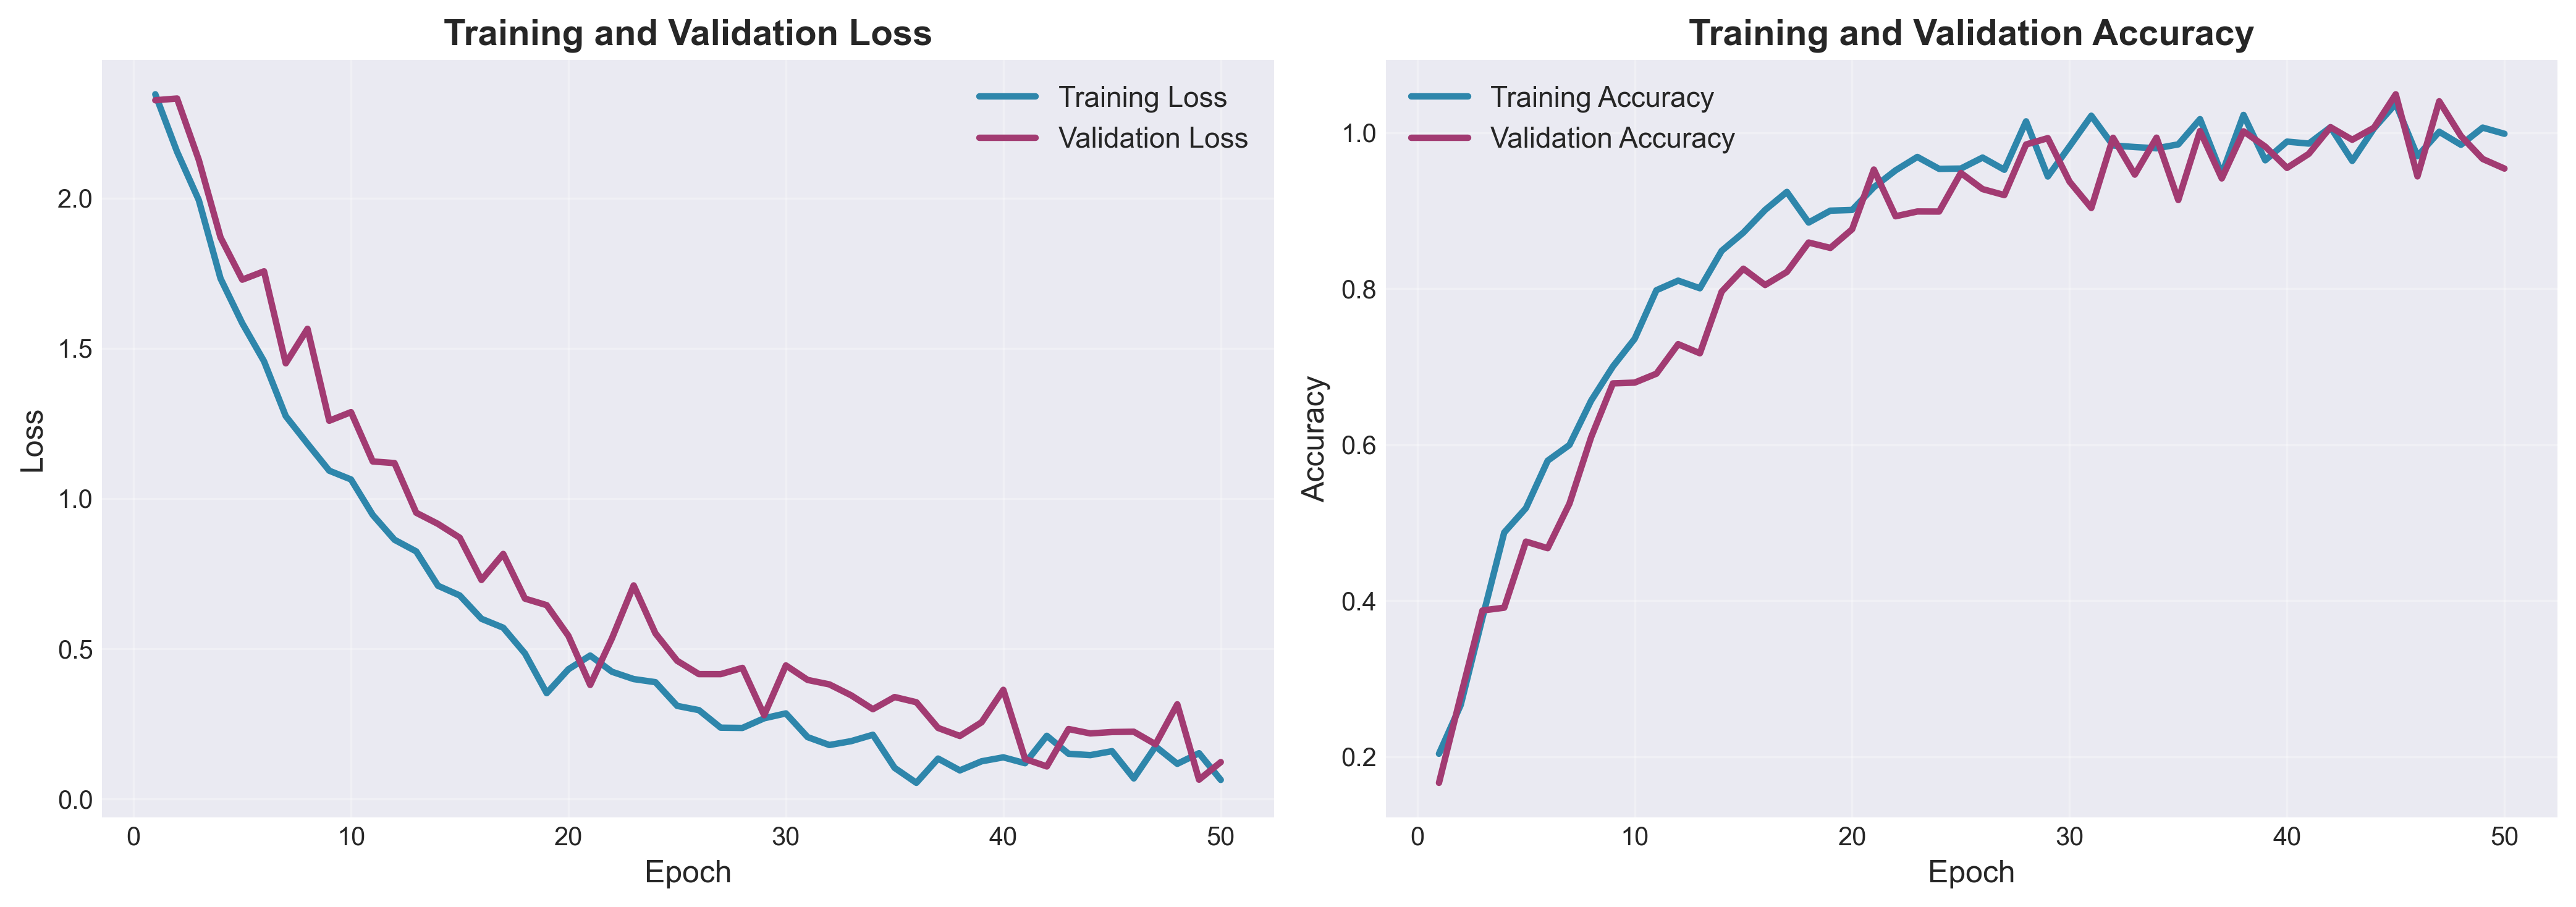
\includegraphics[width=\textwidth]{../figures/10_learning_curves.png}\\
\centering{\small Training and validation learning curves}
\end{columns}
\end{frame}

\begin{frame}{Preprocessing Pipeline}
\begin{columns}
\column{0.5\textwidth}
\textbf{Essential Preprocessing:}
\begin{enumerate}
\item \textbf{Normalization:}
$$x' = \frac{x - \mu}{\sigma}$$

\item \textbf{Standardization:}
$$x' = \frac{x - \text{mean}}{\text{std}}$$

\item \textbf{Rescaling:}
$$x' = \frac{x - x_{\min}}{x_{\max} - x_{\min}}$$
\end{enumerate}

\textbf{Common Schemes:}
\begin{itemize}
\item ImageNet mean/std
\item Scale to [0,1] or [-1,1]
\end{itemize}

\column{0.45\textwidth}
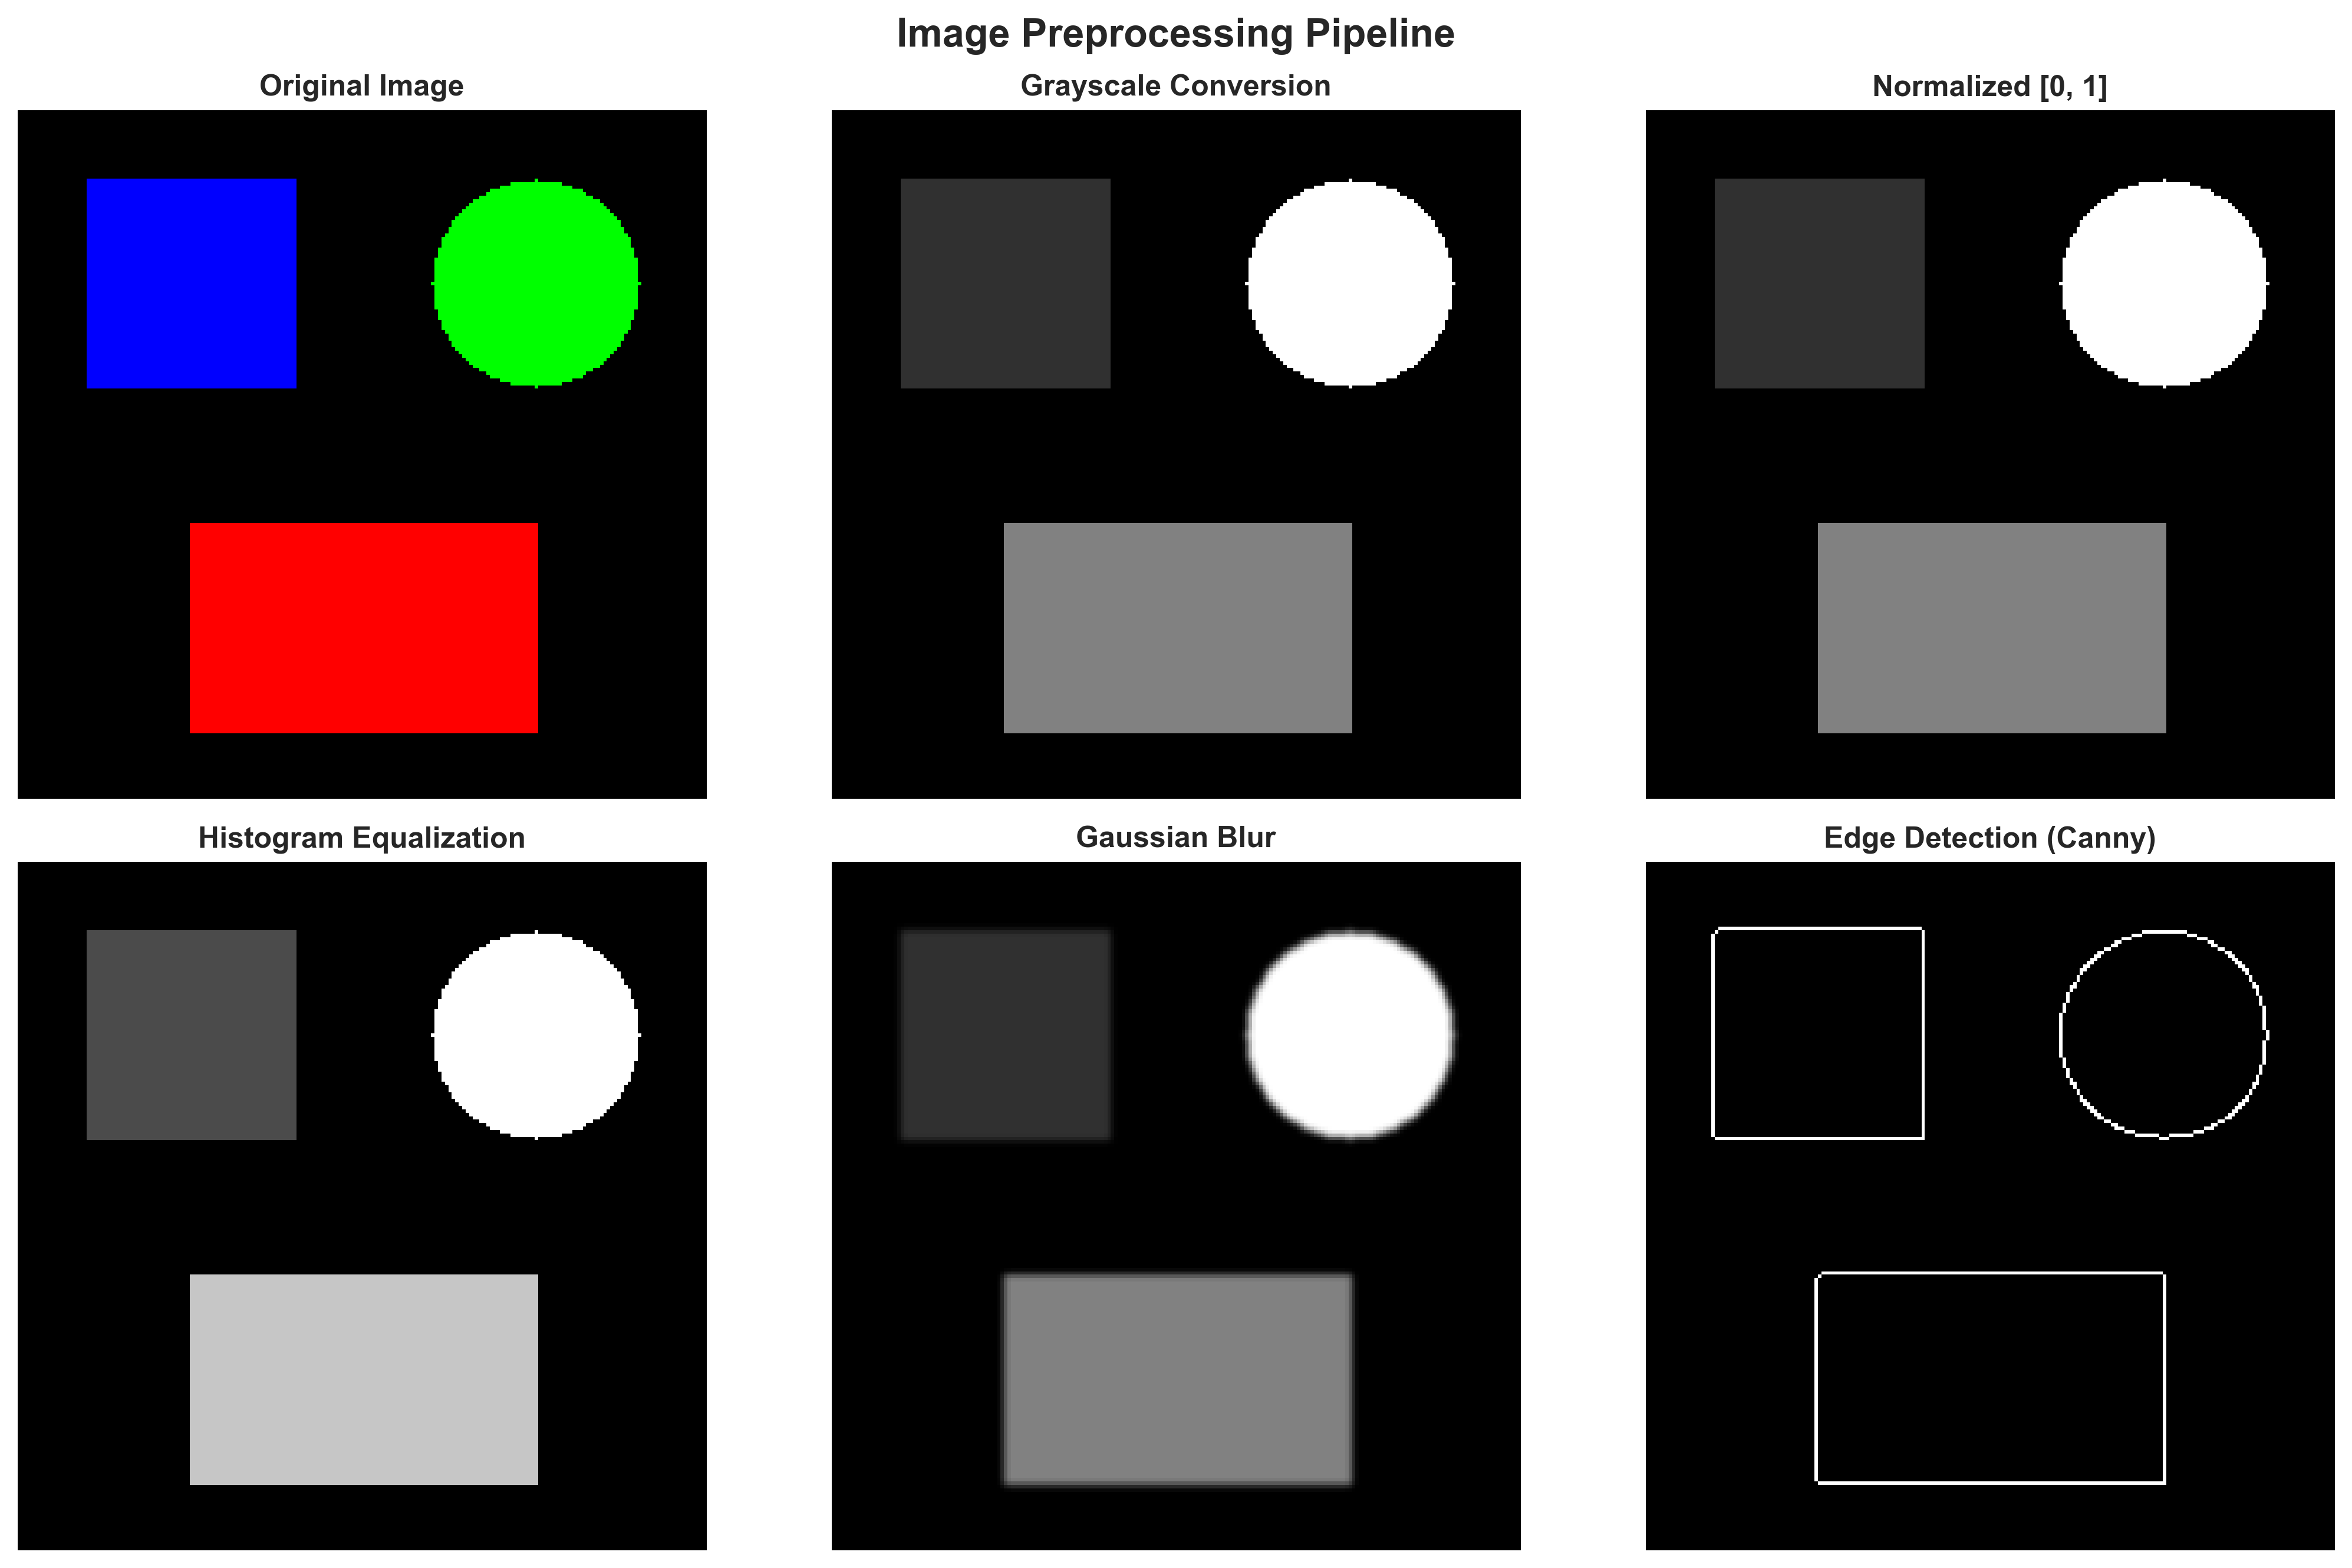
\includegraphics[width=\textwidth]{../figures/11_preprocessing_pipeline.png}\\
\centering{\small Preprocessing pipeline}
\end{columns}
\end{frame}

\begin{frame}{Batch Normalization}
\textbf{Motivation:}
\begin{itemize}
\item Stabilize training and allow higher learning rates
\item Reduce internal covariate shift
\end{itemize}

\textbf{Algorithm:}
\begin{align}
\mu_B &= \frac{1}{m}\sum_{i=1}^{m} x_i \\
\sigma_B^2 &= \frac{1}{m}\sum_{i=1}^{m} (x_i - \mu_B)^2 \\
\hat{x}_i &= \frac{x_i - \mu_B}{\sqrt{\sigma_B^2 + \epsilon}} \\
y_i &= \gamma \hat{x}_i + \beta
\end{align}

Where $\gamma, \beta$ are learnable parameters.
\end{frame}

\section{Overfitting and Regularization}

\begin{frame}{Understanding Overfitting}
\begin{columns}
\column{0.5\textwidth}
\begin{alertblock}{Overfitting}
Model performs well on training data but poorly on test data due to memorizing noise.
\end{alertblock}

\textbf{Causes:}
\begin{itemize}
\item Too many parameters
\item Insufficient training data
\item Lack of regularization
\end{itemize}

\textbf{Signs:}
\begin{itemize}
\item Large gap between train/val loss
\item Decreasing val accuracy
\end{itemize}

\column{0.45\textwidth}
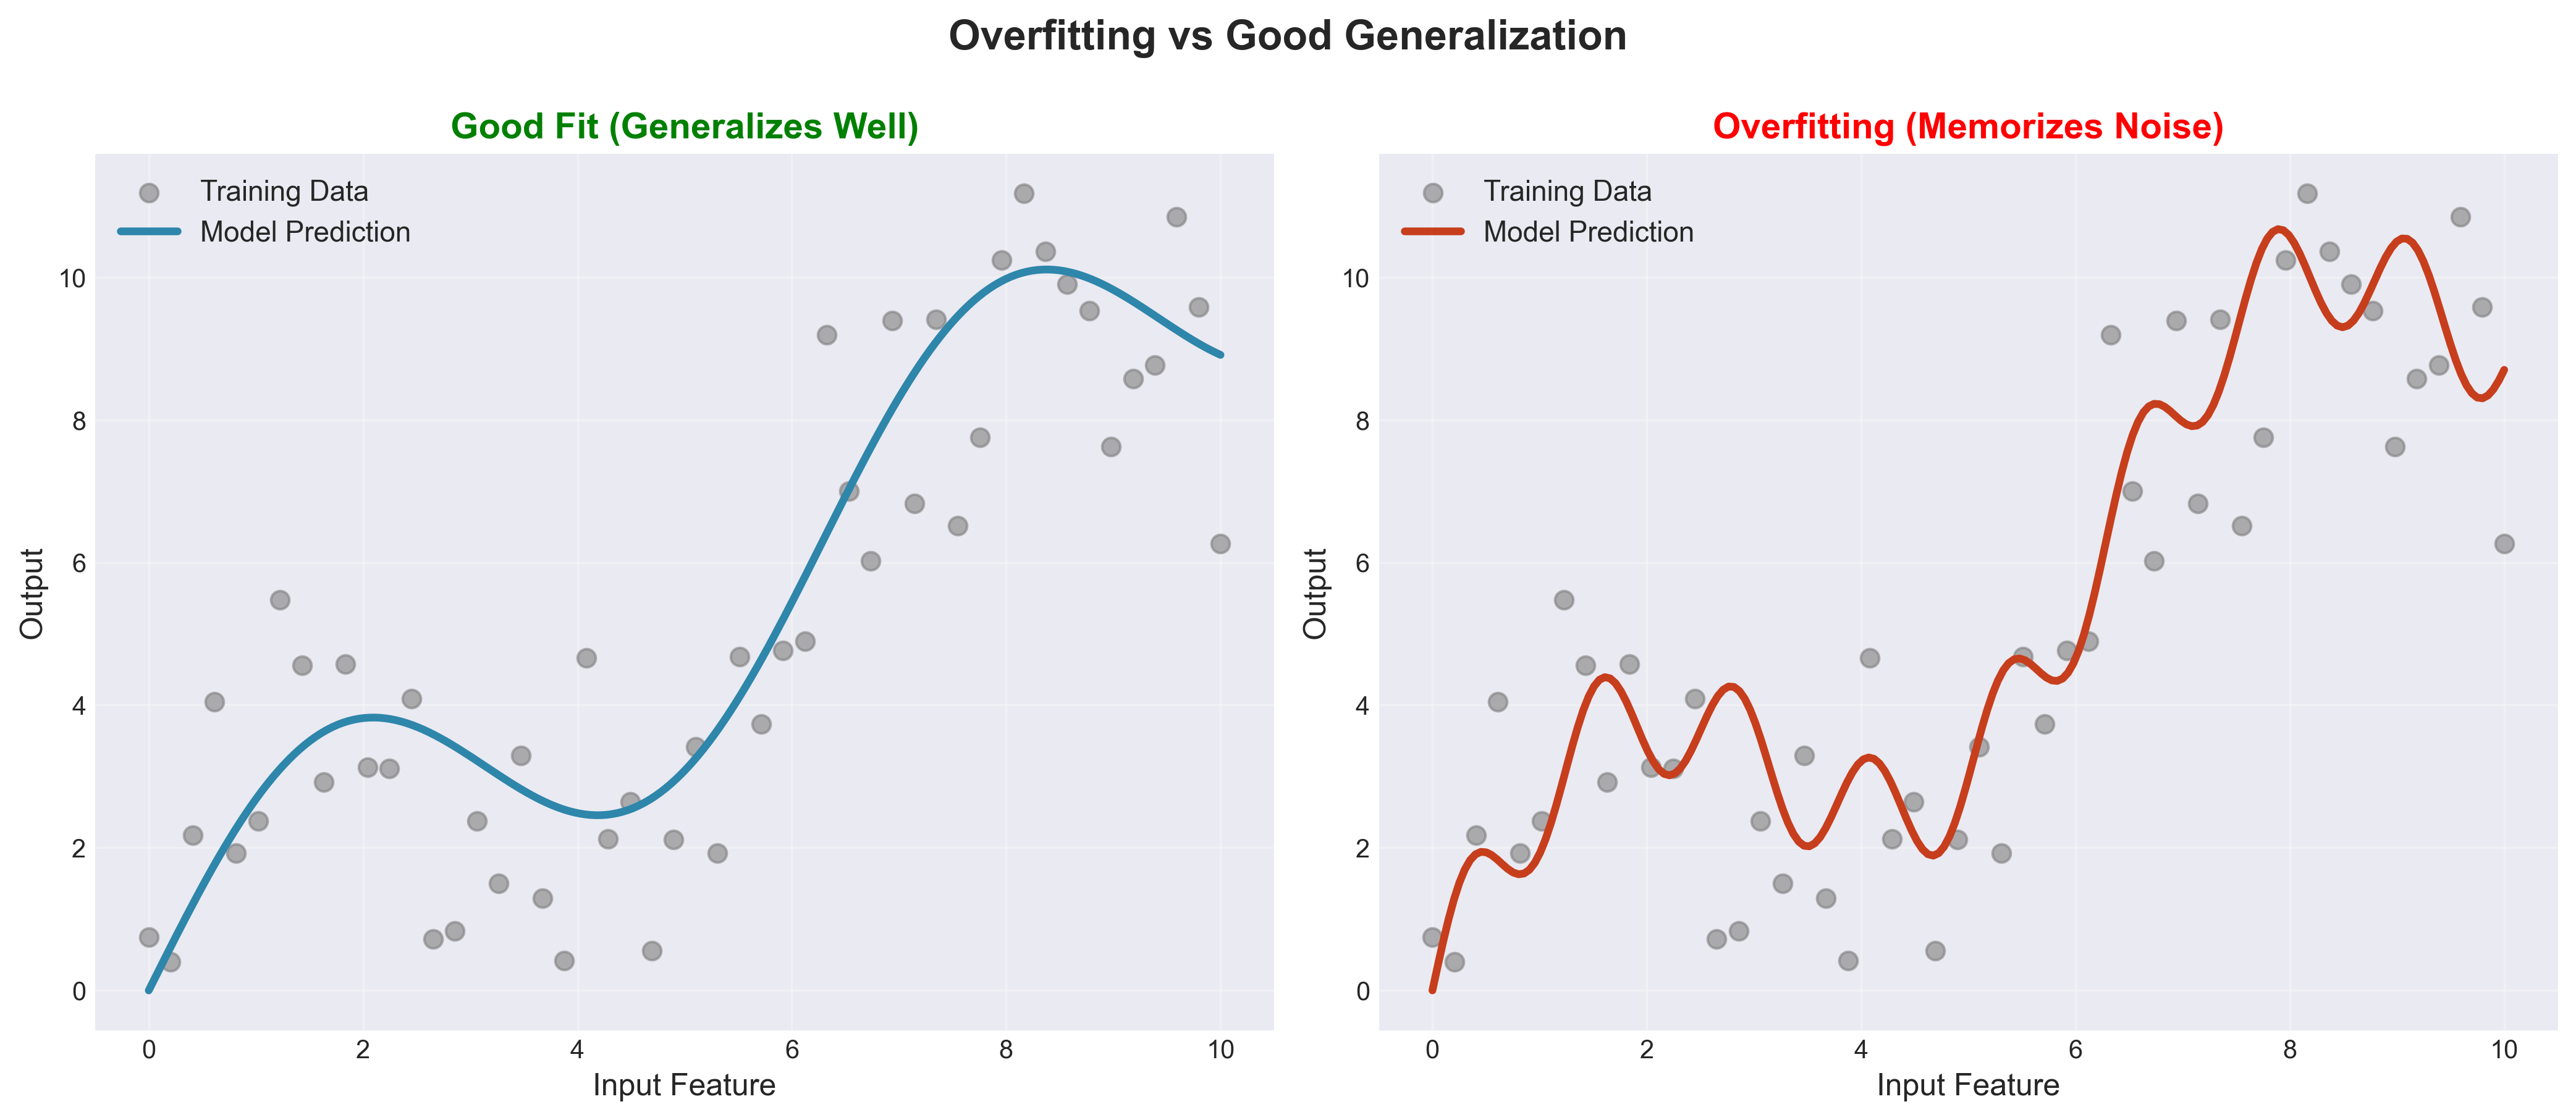
\includegraphics[width=\textwidth]{../figures/15_overfitting_example.png}\\
\centering{\small Overfitting visualization}
\end{columns}
\end{frame}

\begin{frame}{Regularization Techniques}
\textbf{L2 Regularization (Weight Decay):}
$$\mathcal{L}_{\text{total}} = \mathcal{L}_{\text{data}} + \lambda \sum_{i} w_i^2$$

\textbf{L1 Regularization:}
$$\mathcal{L}_{\text{total}} = \mathcal{L}_{\text{data}} + \lambda \sum_{i} |w_i|$$

\textbf{Dropout:}
\begin{itemize}
\item Randomly drop neurons during training (probability $p \approx 0.5$)
\item Forces redundant representations
\item Ensemble effect
\end{itemize}

\textbf{Early Stopping:}
Stop training when validation loss increases
\end{frame}

\begin{frame}{Dropout in Detail}
\textbf{Training Phase:}
$$h_i' = \begin{cases} 0 & \text{with probability } p \\ \frac{h_i}{1-p} & \text{with probability } 1-p \end{cases}$$

\textbf{Test Phase:} Use all neurons (no dropout), activations already scaled

\textbf{Benefits:}
\begin{itemize}
\item Prevents co-adaptation of neurons
\item Implicit ensemble of networks
\item Reduces overfitting significantly
\end{itemize}

\textbf{Typical Values:} 0.5 for hidden layers, 0.2-0.3 for input layers
\end{frame}

\section{Data Augmentation}

\begin{frame}{Data Augmentation Strategies}
\begin{columns}
\column{0.5\textwidth}
\begin{alertblock}{Purpose}
Data augmentation artificially increases training set size by applying label-preserving transformations, improving generalization.
\end{alertblock}

\textbf{Geometric Transformations:}
\begin{itemize}
\item Random rotation
\item Horizontal/vertical flips
\item Random crops
\item Scaling and zooming
\item Shearing and translation
\end{itemize}

\column{0.45\textwidth}
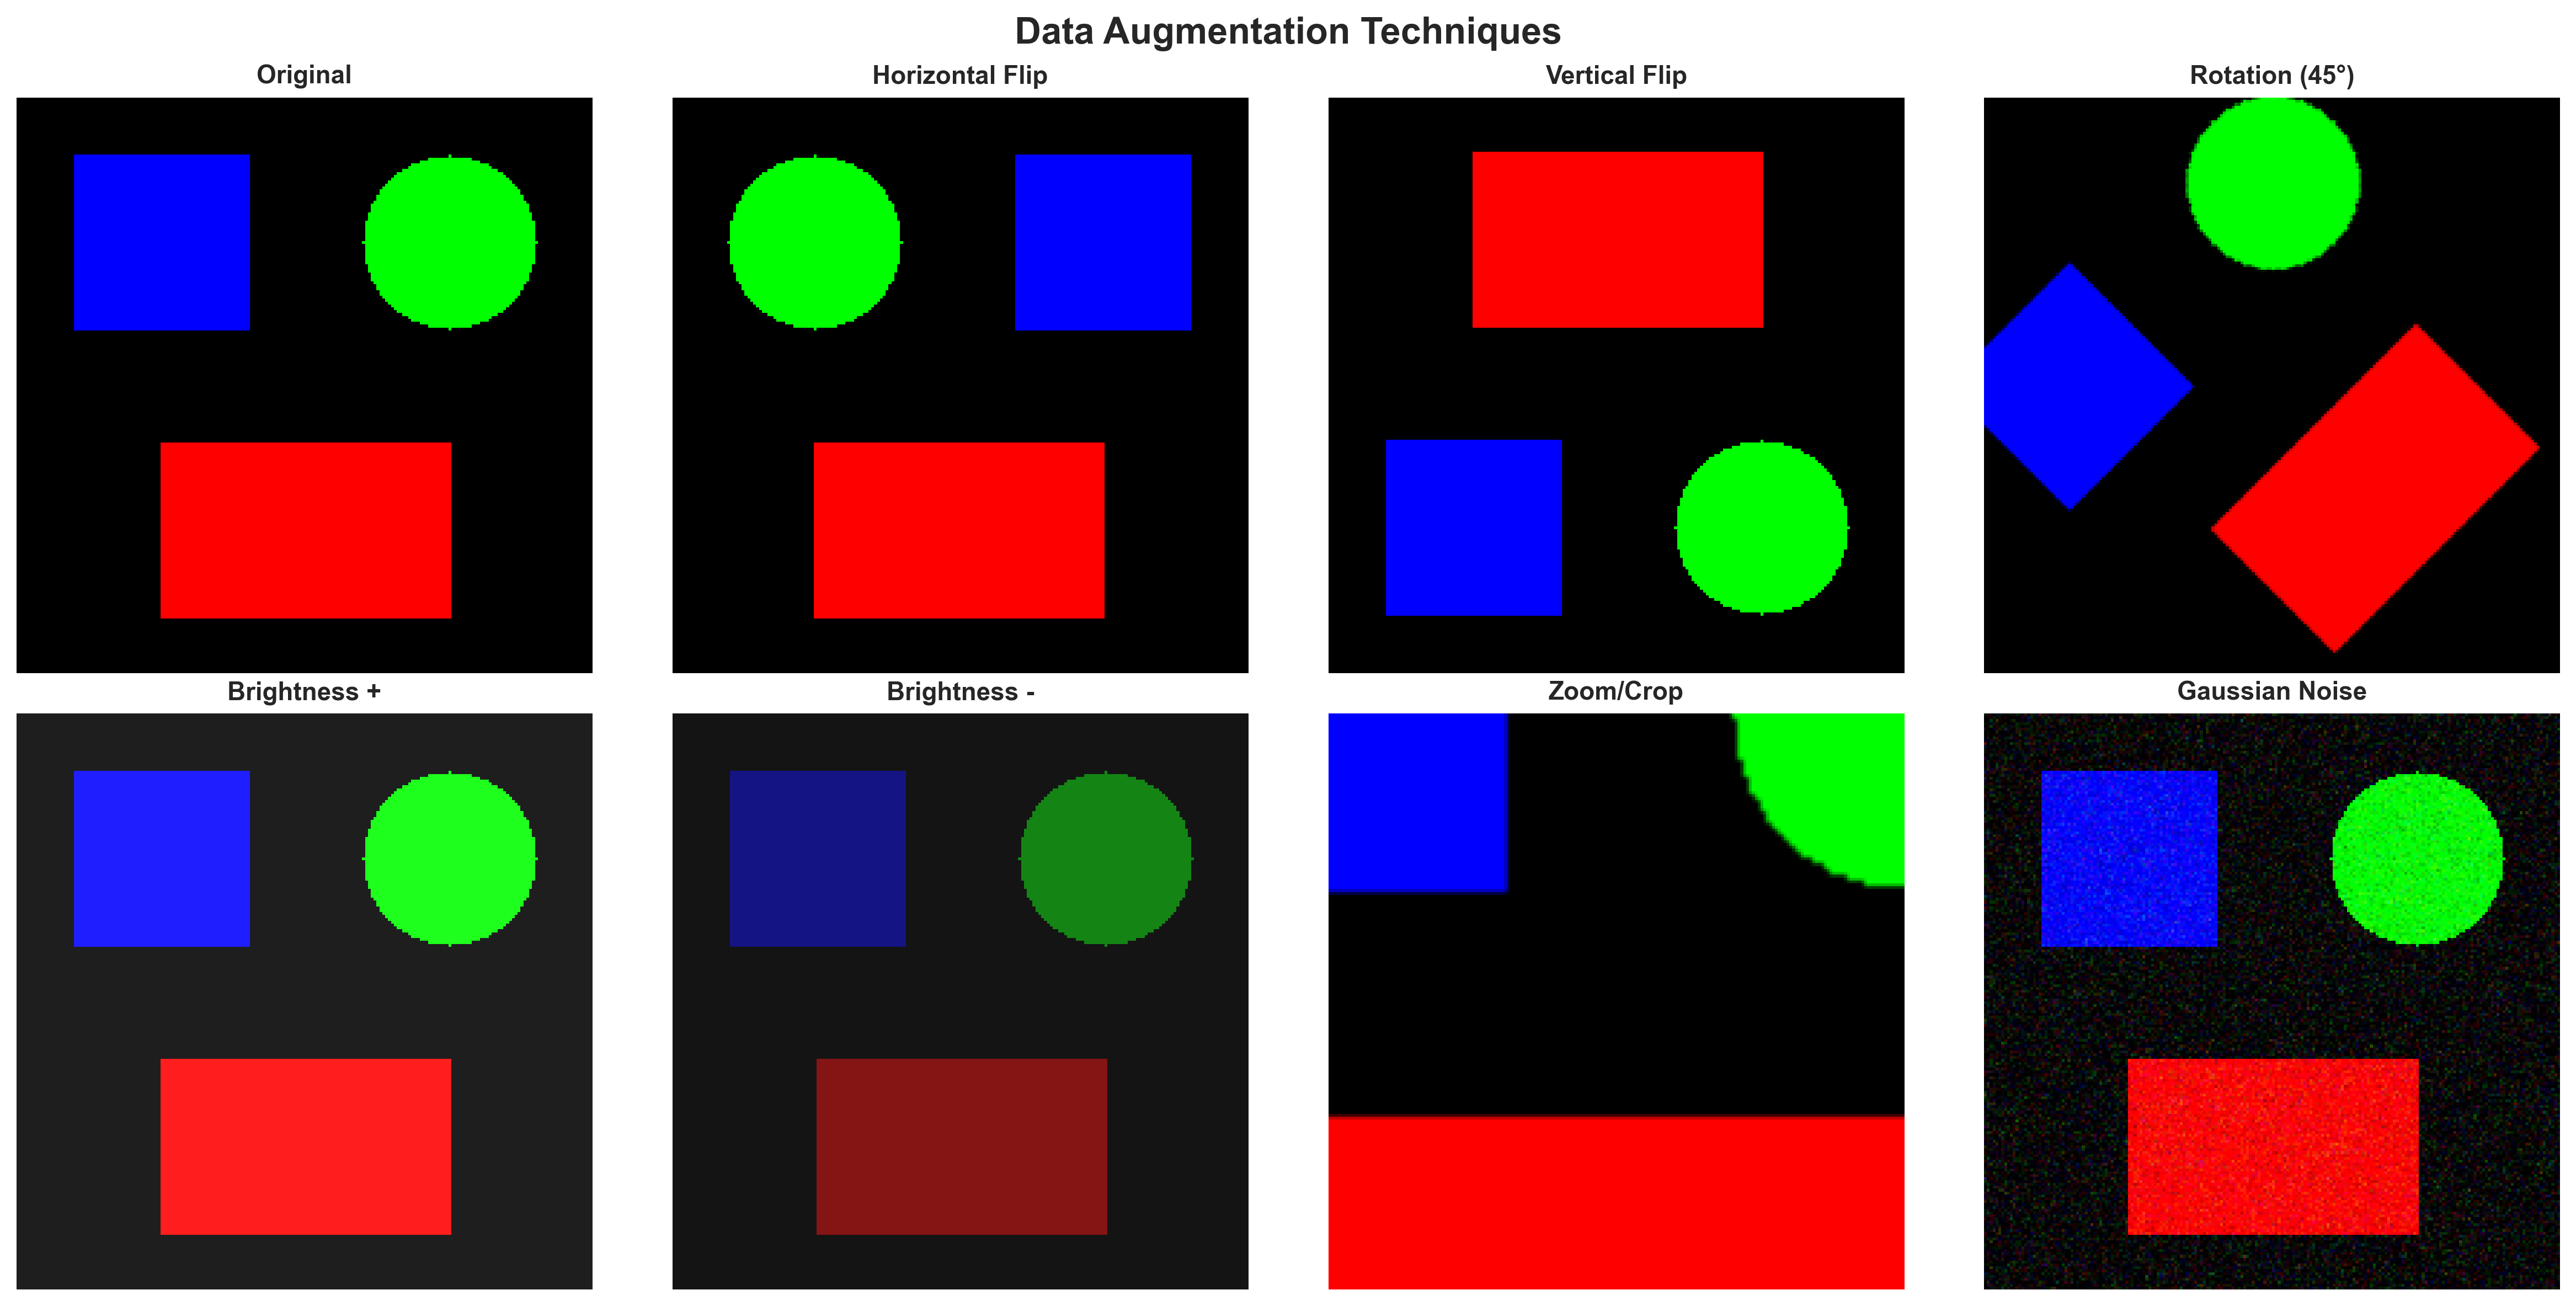
\includegraphics[width=\textwidth]{../figures/12_data_augmentation.png}\\
\centering{\small Various data augmentation techniques}
\end{columns}
\end{frame}

\begin{frame}{Advanced Augmentation}
\textbf{Color-based Augmentation:}
\begin{itemize}
\item Brightness, contrast, saturation
\item Hue shifts and noise injection
\end{itemize}

\textbf{Modern Techniques:}
\begin{itemize}
\item \textbf{Cutout:} Random rectangular occlusion
\item \textbf{Mixup:} Linear interpolation between samples
\item \textbf{CutMix:} Replace image regions between samples
\item \textbf{AutoAugment:} Learned augmentation policies
\end{itemize}

\textbf{Best Practices:}
\begin{itemize}
\item Apply augmentation online during training
\item Use task-appropriate transformations
\item Combine multiple augmentations
\end{itemize}
\end{frame}

\section{Transfer Learning}

\begin{frame}{Transfer Learning Basics}
\begin{alertblock}{Core Concept}
Transfer learning leverages knowledge learned from one task to improve performance on a related task, especially valuable with limited training data.
\end{alertblock}

\textbf{Why Transfer Learning?}
\begin{itemize}
\item Training from scratch requires massive datasets
\item Pre-trained models capture general features
\item Faster convergence
\item Better performance with less data
\end{itemize}

\textbf{Common Approach:}
\begin{enumerate}
\item Start with pre-trained model (e.g., ImageNet)
\item Remove final classification layer
\item Add new layers for target task
\item Fine-tune on target dataset
\end{enumerate}
\end{frame}

\begin{frame}{Transfer Learning Strategies}
\textbf{Feature Extraction:}
\begin{itemize}
\item Freeze pre-trained layers, train only new layers
\item Fast and stable, good for small datasets
\end{itemize}

\textbf{Fine-tuning:}
\begin{itemize}
\item Unfreeze some/all layers
\item Train with lower learning rate
\item Better performance, requires more data
\end{itemize}

\textbf{Layer-wise Strategy:}
\begin{itemize}
\item Early layers: Generic features (edges, textures)
\item Later layers: Task-specific features
\item Fine-tune later layers first, then gradually unfreeze earlier layers
\end{itemize}
\end{frame}

\begin{frame}{Practical Transfer Learning}
\textbf{Learning Rate Strategy:}
\begin{itemize}
\item Pre-trained layers: $\eta = 10^{-5}$ to $10^{-4}$
\item New layers: $\eta = 10^{-3}$ to $10^{-2}$
\item Use different learning rates for different layer groups
\end{itemize}

\textbf{Decision Tree:}
\begin{itemize}
\item \textbf{Small dataset + Similar task:} Feature extraction
\item \textbf{Small dataset + Different task:} Fine-tune top layers
\item \textbf{Large dataset + Similar task:} Fine-tune all layers
\item \textbf{Large dataset + Different task:} Train from scratch or fine-tune extensively
\end{itemize}

\textbf{Popular Pre-trained Models:}
\begin{itemize}
\item ResNet, VGG, Inception (ImageNet)
\item EfficientNet, MobileNet (efficiency-focused)
\end{itemize}
\end{frame}

\section{Evaluation and Metrics}

\begin{frame}{Classification Metrics}
\begin{columns}
\column{0.5\textwidth}
\textbf{Confusion Matrix:}
\begin{itemize}
\item True Positives (TP)
\item False Positives (FP)
\item True Negatives (TN)
\item False Negatives (FN)
\end{itemize}

\textbf{Derived Metrics:}
\begin{align}
\text{Accuracy} &= \frac{TP + TN}{TP + TN + FP + FN} \\
\text{Precision} &= \frac{TP}{TP + FP} \\
\text{Recall} &= \frac{TP}{TP + FN} \\
\text{F1} &= 2 \cdot \frac{\text{Prec} \cdot \text{Rec}}{\text{Prec} + \text{Rec}}
\end{align}

\column{0.45\textwidth}
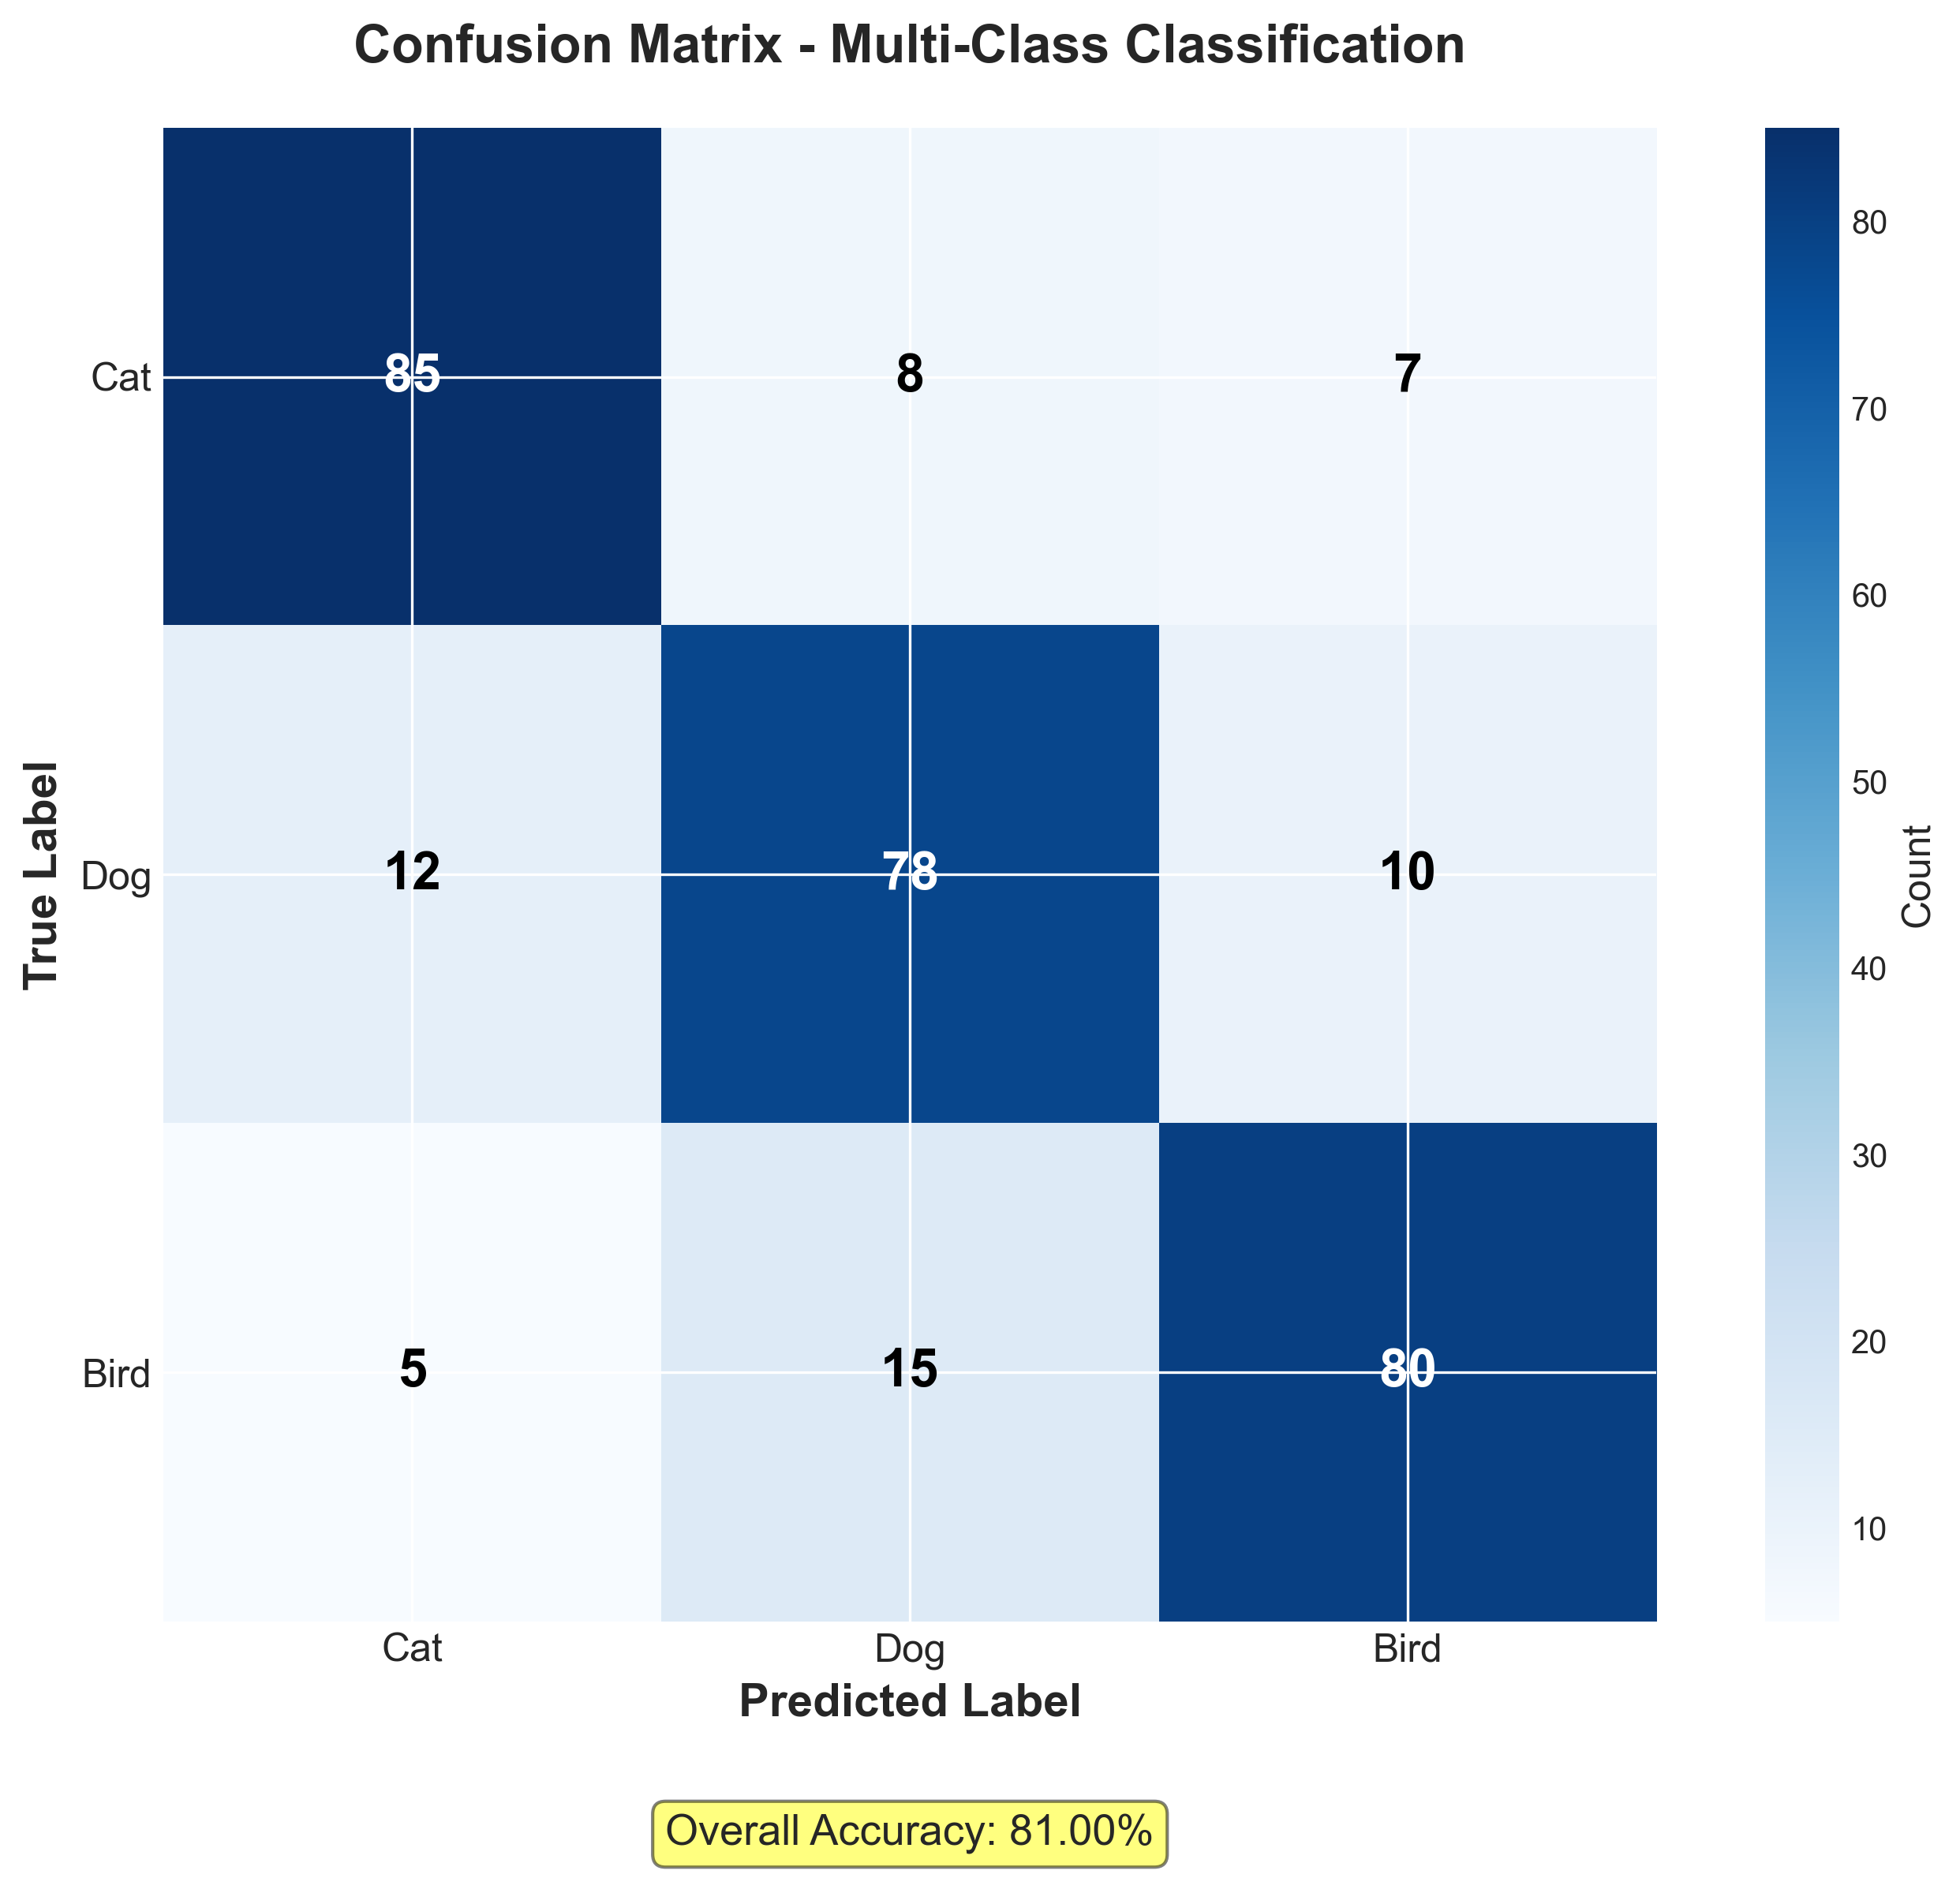
\includegraphics[width=\textwidth]{../figures/14_confusion_matrix.png}\\
\centering{\small Confusion matrix for multi-class classification}
\end{columns}
\end{frame}

\begin{frame}{Model Evaluation Best Practices}
\textbf{Data Splitting:}
\begin{itemize}
\item \textbf{Training set:} 60-80\% for learning
\item \textbf{Validation set:} 10-20\% for tuning
\item \textbf{Test set:} 10-20\% for final evaluation
\end{itemize}

\textbf{Cross-validation:}
\begin{itemize}
\item K-fold CV for robust estimates
\item Stratified sampling for imbalanced data
\item Use when data is limited
\end{itemize}

\textbf{Monitoring:}
\begin{itemize}
\item Track train/val loss and accuracy
\item Visualize learning curves
\item Check for overfitting/underfitting
\item Monitor gradient norms
\end{itemize}
\end{frame}

\section{Best Practices}

\begin{frame}{Training Best Practices}
\textbf{Initialization:}
\begin{itemize}
\item Use proper weight initialization (Xavier, He)
\item Initialize biases to zero, never same values for all weights
\end{itemize}

\textbf{Optimization:}
\begin{itemize}
\item Start with Adam optimizer
\item Use learning rate scheduling
\item Gradient clipping for stability
\end{itemize}

\textbf{Regularization:}
\begin{itemize}
\item Apply dropout (0.5 for FC layers)
\item Use weight decay ($\lambda = 10^{-4}$ to $10^{-5}$)
\item Batch normalization for deep networks
\item Data augmentation as primary regularizer
\end{itemize}
\end{frame}

\begin{frame}{Debugging Neural Networks - Part 1}
\textbf{Common Issues and Solutions:}

\begin{alertblock}{Loss not decreasing}
\begin{itemize}
\item Check learning rate (too high/low)
\item Verify data preprocessing
\item Check for bugs in loss computation
\end{itemize}
\end{alertblock}

\begin{alertblock}{Validation accuracy not improving}
\begin{itemize}
\item Model too simple (increase capacity)
\item Poor hyperparameters
\item Insufficient training time
\end{itemize}
\end{alertblock}
\end{frame}

\begin{frame}{Debugging Neural Networks - Part 2}
\begin{alertblock}{NaN/Inf values}
\begin{itemize}
\item Gradient explosion (reduce learning rate)
\item Numerical instability (check activations)
\item Division by zero (check loss function)
\end{itemize}
\end{alertblock}

\textbf{Additional Debugging Tips:}
\begin{itemize}
\item Start with a small dataset to verify pipeline
\item Check gradients are flowing properly
\item Monitor activation distributions
\item Validate data augmentation is working correctly
\end{itemize}
\end{frame}

\begin{frame}{Hyperparameter Tuning - Priority}
\textbf{Priority Order:}
\begin{enumerate}
\item \textbf{Learning rate:} Most important
\item \textbf{Architecture:} Depth, width
\item \textbf{Batch size:} 32, 64, 128, 256
\item \textbf{Regularization:} Dropout, weight decay
\item \textbf{Optimizer:} Adam, SGD+Momentum
\end{enumerate}

\textbf{Search Strategies:}
\begin{itemize}
\item \textbf{Grid search:} Systematic, exhaustive
\item \textbf{Random search:} Often more efficient
\item \textbf{Bayesian optimization:} Smart sampling
\item \textbf{Manual tuning:} Domain expertise
\end{itemize}
\end{frame}

\begin{frame}{Learning Rate Finding}
\textbf{Learning Rate Finding Technique:}
\begin{enumerate}
\item Start very small ($10^{-6}$)
\item Gradually increase learning rate
\item Stop when loss diverges
\item Use point before divergence
\end{enumerate}

\textbf{Best Practices:}
\begin{itemize}
\item Use learning rate warmup for stability
\item Consider cyclical learning rates
\item Monitor both training and validation metrics
\item Adjust based on gradient norms
\end{itemize}
\end{frame}

\section{Summary}

\begin{frame}{Key Takeaways - Fundamentals}
\textbf{Neural Network Basics:}
\begin{itemize}
\item Perceptrons are building blocks
\item Activation functions enable non-linearity
\item Backpropagation efficiently computes gradients
\item Optimization guides learning process
\end{itemize}

\textbf{Loss and Optimization:}
\begin{itemize}
\item MSE for regression, Cross-entropy for classification
\item Adam optimizer often best starting point
\item Learning rate is critical hyperparameter
\item Momentum accelerates convergence
\end{itemize}
\end{frame}

\begin{frame}{Key Takeaways - CNNs}
\textbf{Convolutional Networks:}
\begin{itemize}
\item Leverage spatial structure of images
\item Convolution extracts local features
\item Pooling provides invariance and reduction
\item Hierarchical feature learning
\end{itemize}

\textbf{Architecture Design:}
\begin{itemize}
\item Deeper networks learn better representations
\item Residual connections enable very deep networks
\item Balance between depth and width
\item Pre-trained models accelerate development
\end{itemize}
\end{frame}

\begin{frame}{Key Takeaways - Training}
\textbf{Practical Training:}
\begin{itemize}
\item Proper preprocessing is essential
\item Data augmentation improves generalization
\item Monitor train/val metrics closely
\item Regularization prevents overfitting
\end{itemize}

\textbf{Best Practices:}
\begin{itemize}
\item Start simple, then increase complexity
\item Transfer learning for limited data
\item Systematic hyperparameter tuning
\item Validate on held-out test set
\end{itemize}
\end{frame}

\begin{frame}{Next Steps in Deep Learning}
\textbf{Advanced Architectures:}
\begin{itemize}
\item Attention mechanisms and Transformers
\item Object detection (YOLO, R-CNN)
\item Semantic segmentation (U-Net, DeepLab)
\end{itemize}

\textbf{Advanced Topics:}
\begin{itemize}
\item Generative models (GANs, VAEs, Diffusion)
\item Self-supervised and few-shot learning
\item Neural architecture search
\end{itemize}

\textbf{Applications:}
\begin{itemize}
\item Medical image analysis and autonomous driving
\item Face recognition and biometrics
\item Image generation and editing
\end{itemize}
\end{frame}

\begin{frame}[standout]
\Large
\textbf{Questions \& Discussion}

\vspace{1cm}
\normalsize
Ready to build your first CNN?\\
Check out the interactive notebook!
\end{frame}

\end{document}
